\documentclass[UKenglish]{article}

\RequirePackage[no-math]{fontspec}

\usepackage[small]{dgruyter}
\usepackage{microtype}
\usepackage{enumerate}
\usepackage{eqnarray}
\usepackage{colortbl}
\usepackage{soul}

\usepackage[firstpage]{draftwatermark}
\SetWatermarkText{\parbox{12cm}{\centering\sffamily\Large Final draft, to appear in Cognitive Linguistics.\\Please quote as such until publication.\\Please do \textit{not} quote this paper using\\the projected volume\slash issue given here.}}
\SetWatermarkColor{blue}
\SetWatermarkHorCenter{0.65\paperwidth}
\SetWatermarkVerCenter{0.875\paperheight}
\SetWatermarkAngle{0}

\newcommand{\eg}{e.\,g.,}
\newcommand{\Eg}{E.\,g.,}
\newcommand{\ie}{i.\,e.,}
\newcommand{\Ie}{I.\,e.,}
\newcommand{\Sub}[1]{\ensuremath{\mathrm{_{#1}}}}
\newcommand{\Sup}[1]{\ensuremath{\mathrm{^{#1}}}}
\newcommand{\Subsf}[1]{\ensuremath{\mathsf{_{#1}}}}
\newcommand{\Supsf}[1]{\ensuremath{\mathsf{^{#1}}}}
\newcommand{\pPB}{p\Subsf{PB}}
\newcommand{\mpPB}{\ensuremath{p_{\text{PB}}}}

\newcommand{\NACb}{NAC\Sub{bare}}
\newcommand{\NACa}{NAC\Sub{adj}}
\newcommand{\PGCd}{PGC\Sub{det}}
\newcommand{\PGCa}{PGC\Sub{adj}}

\newcommand*\Rot{\rotatebox{75}}

\definecolor{lg}{rgb}{.8,.8,.8}
\newcommand{\Dim}{\cellcolor{lg}}

\usepackage{gb4e-}

\usepackage{bbding}
\newcommand{\CheckIt}{\CheckmarkBold}
\newcommand{\CrossIt}{\XSolidBold}


\usepackage{natbib}
\bibliographystyle{./unified}

\usepackage{lineno}

\begin{document}

  %\articletype{...}

  \author*[1]{Roland Schäfer}
  \runningauthor{Roland Schäfer}
  \affil[1]{Deutsche und niederländische Philologie, Freie Universität Berlin, email: roland.schaefer@fu-berlin.de}

  \title{Abstractions and exemplars: the measure noun phrase alternation in German}
  \runningtitle{Abstraction and exemplars: the measure noun phrase alternation German}
  %\subtitle{...}

  \abstract{In this paper, an alternation in German measure noun phrases is examined under a varying-abstraction perspective.
    In a specific measure NP construction, the embedded kind-denoting noun either agrees in case with the measure noun (\textit{eine Tasse guter Kaffee} `a cup of good coffee') or it stands in the genitive (\textit{eine Tasse guten Kaffees}).
    Each of the two alternants is syntactically similar to a non-alternating construction.
    I propose a prototype model which assigns a common prototypical meaning to each of the alternants and its corresponding non-alternating construction.
    Based on this, I argue that lexical, morpho-syntactic, and stylistic features help to predict the choice of the alternant.
    A large corpus study is presented which supports this analysis.
    However, in addition to the prototype effects, an exemplar effect is also shown to influence the choice, namely the relative frequencies with which lemmas occur in the non-alternating constructions.
    I argue that allowing both prototype and exemplar effects is more adequate than following radical prototype or exemplar approaches.
    It is also verified in two experiments that the corpus-derived model corresponds to the behaviour of native speakers.
    The weak effect size of the experimental validation is discussed in the context of corpus-based cognitive linguistics and the validation of corpus-derived models.}
  \keywords{prototypes vs.\ exemplars, corpus methods and experimental validation, morpho-syntactic alternations, multilevel modeling, pseudo-partitives, German}
  %\classification[PACS]{...}
  %\communicated{...}
  %\dedication{...}
  \received{18 April 2017}
  \accepted{31 May 2018}
  \journalname{Cognitive Linguistics}
  \journalyear{2018}
  \journalvolume{4}
  \journalissue{29}
  \startpage{10000}
  %\aop
  %\DOI{...}

  
\maketitle


\section{Prototypes, exemplars, and corpora in cognitive linguistics}
\label{sec:cogocl}

This paper deals with a morpho-syntactic alternation between two constructions which occurs only in a very specific type of measure noun phrase in German.
By \textit{alternation} I refer to a situation where two or more forms or constructions are available with no clear (but potentially a subtle) difference in acceptability, function, or meaning.
The study of lexical and constructional alternations has a long history in cognitively oriented corpus linguistics (for example, \citealp{BresnanEa2007,BresnanHay2010,BresnanFord2010,DivjakArppe2013,Gries2015,NessetJanda2010}).
This area of research is based on the assumption that language is a probabilistic phenomenon \citep{Bresnan2007} where alternants are chosen neither deterministically nor fully at random.
Instead, multifactorial models are constructed which incorporate influencing factors from diverse levels, including lexical and contextual factors.
The estimation of the model coefficients quantifies the influence that the factors have on the probability that either alternant is chosen.
There are two fundamental issues to consider with respect to this tradition as a part of cognitive linguistics in the broad sense.
First, there is the question of whether corpus data do provide any insight into cognitive representations at all.
This question can and should be answered by testing how well corpus-derived models converge with or diverge from experimental findings, which provide more direct evidence of mental representations and processes but are often intrinsically narrower in scope.
Second and closely related to the first question, the appropriate modelling of such results in cognitive linguistics (\ie\ the assumed underlying constructs) is a key issue.

Concerning the first point, there has for a long time been an interest in correlating probabilistic generalisations extracted from corpus data with results from experimental work (for example, \citealp{ArppeJaervikivi2007,BresnanEa2007,BresnanFord2010,DivjakGries2008,DivjakEa2016,FordBresnan2013}).
This is often called a \textit{validation} of the corpus-derived findings, but \citet[303]{Divjak2016a} criticises this choice of words ``because it creates the impression that behavioral experimental data is inherently more valuable than textual data'', citing \cite{TummersEa2005}, who state that a corpus is ``a sample of spontaneous language use that is (generally) realized by native speakers''.
See also \citet{Newman2011} for a very positive view of corpora as a source of data in cognitive linguistics in their own right.
However, as \citet[486--487]{Dabrowska2016} convincingly argues, this does not mean that we can in some way ``deduce mental representations from patterns of use'', \ie\ from corpus data.
It would be highly surprising if this were possible, and the same holds for experimental methods, albeit to a different degree.
Nobody assumes that we can inductively infer mental representations from experiments, which -- as opposed to corpus studies -- even allow for direct access to the cognitive agent and offer much better possibilities to control experimental conditions and nuisance variables.
Rather, a theory of cognitive representation is pre-specified.
Then, predictions are derived from this theory \textit{before} the experiment or the corpus study is conducted in order to \textit{test} the theory.
While the same approach is by and large applicable to corpus data, I now discuss some relevant differences.

As mentioned above, the central question is whether usage data as found in corpora are truly predictive of speakers' and writers' cognitive representation of language and\slash or of their overall linguistic behaviour; and this is where the experimental validation (or, more neutrally, \textit{corroboration}) comes into play.
An overview of this issue was given by \cite{NewmanSorensenduncan2015}, who enumerate a number of studies which show how corpus data and experimental data converge (such as \citealp{BresnanEa2007,DurrantDoherty2010,GriesWulff2005,GriesEa2005}) and a number of studies where the two types of data led to diverging or only partially converging results (such as \citealp{ArppeJaervikivi2007,Dabrowska2014,Mollin2009}).
When researchers do not achieve convergence, they mostly try to explain this by differentiating between the actual cognitive construct and what the pooled usage data as found in corpora represent.
For example, \citet[411]{Dabrowska2014} lists a long number of possible reasons to explain why subjects in her experiment diverged in their word association preferences from collocation measures extracted from corpora.
In some cases, researchers simply argue for a more adequate statistical analysis to increase the fit between corpus data and subjects' reactions in experiments, for example \cite{DivjakEa2016}, who show that generalised additive models (GAMs) are better suited than generalised linear models (GLMs) in the analysis of their reading-time experiment based on data extracted from previous corpus studies.
Much more optimistically compared to these publications dealing with possible frictions between usage and experimental data, \cite{StefanowitschFlach2016} recently proposed a straightforward positivist perspective of corpora as representing the input of an average adult speaker, thus licensing inferences from corpus data to cognitive representations learned from such data under a ``corpus-as-input'' view.
They state that ``in this wider context, large, register-mixed corpora such as the British National Corpus [\ldots] may not be perfect models of the linguistic experience of adult speakers, but they are reasonably close to the input of an idealized average member of the relevant speech community'' \citep[104]{StefanowitschFlach2016}.
In essence, this would entail that any generalisation extracted from the BNC could be assumed to have some kind of mental reality, which is at least doubtful.

Obviously, no clear picture has emerged yet, which is not surprising given the vast number of cognitive constructs assumed at diverse levels (such as the level of words in collocation research and much more complex constructional levels in alternation research involving lexical, syntagmatic, and contextual factors), the problems of corpus composition, the operationalisations involved in making experiments, and the choice of statistical tools.
While far from providing definitive solutions, my discussion in Section~\ref{sec:conclusion} will provide possible explanations for the goodness of fit between the corpus data and the experimental data reported in Sections~\ref{sec:corpusstudies} and~\ref{sec:experimental}, much in the spirit of \citet{Dabrowska2014}.

I now turn to the second issue, namely which type of cognitive representation research on alternations provides evidence for.
The typical approach in alternation research is to annotate a large number of corpus sentences with linguistic features and to model the probability of the variants being chosen given these features.
The idea is that a variant is chosen when the influencing features cumulatively assume typical values for that variant.
In other words, a variant of prototype theory with features \citep{Rosch1978} is the appropriate model, also because the features used to feed the model are more often than not abstract high-level linguistic features. 
Some researchers such as \cite{Gries2003}, \cite{NessetJanda2010}, or \cite{Schaefer2016c} indeed commit to prototype theory in alternation modelling.
Under prototype theory, category membership is defined by similarity to an ideal exemplar, which is usually identified with characterising features (see \citealp{Taylor2008} for an overview).
While prototype theory is well suited for modeling constructional choices, it is just one of at least two major similarity-based theories of classification, the most prominent other framework being exemplar theory (\citealp{MedinSchaffer1978,Hintzman1986}).
Prototype theory and exemplar theory model essentially the same types of effects when only output data are considered.
Corpus data (representing purely output data, usually from many speakers) might serve as evidence that some form of similarity-based classification is appropriate.
However, the theories differ significantly in whether they assume higher-level abstractions in the form of single maximally prototypical exemplars or their features (prototype theory) or assume that categories emerge through the storage of many exemplars and similarity classification on those exemplars (exemplar theory).
Similarity-based categorisation is seen as the central and conceptually sufficient approach to linguistic categorisation by many cognitive linguists.
For example, see \cite{Taylor2003} for a comprehensive treatment in terms of prototype theory and \cite{Taylor2012} for a detailed discussion of an exemplar-based approach.
In the influential framework of cognitive grammar \citep{Langacker1987}, prototypes (which, as should be remembered, represent abstractions already in cognitive science) are literally taken as prototypical exemplars, and there is an additional level of fully discrete abstractions in the form of schemas.
Schemas are characterised by the properties common to all members of the category, whereas a prototypical category member might have very specific additional properties not at all shared by all or even most members \citep[371-375]{Langacker1987}.
The prototype can serve as a reference point when classifying new objects which do not share all properties of the schema, but this would (if repeated) lead to the creation of an even more abstract (hierarchically higher and less specific) schema which describes the new member and the ones belonging to the previous schema.
As pointed out by \citet[136--137]{Langacker1987}, schemas and prototypes thus fulfil different roles and can be assumed to co-exist.
A strict exemplar view of language is incompatible, as far as I can see, with Langacker's view of schemas, but any theory of categorisation that allows for at least some kind of abstraction, is not in principled contradiction with it.
In the remainder of this paper, I do not use schemas in my descriptions of the relevant categories, mostly because the aspect of similarity and fuzzy classification is central to my point, and a formulation in terms of schemas would bring about an unnecessarily high degree of abstraction (see \citealp[70--71]{Taylor2003} for a parallel argument).
However, I fully describe the abstract features of the prototypes.

Turning back to the prototype vs.\ exemplar debate, \cite{Barsalou1990} already showed that prototype and exemplar theory model the same types of effects and are informationally equivalent.
Consequently, experiments which favour one theory over the other use procedural behaviour of subjects in experiments, for example the speed of category retrieval, as opposed to mere output data.
In very early experiments, \cite{PosnerKeele1968} showed, for example, that highly prototypical unseen exemplars were categorised more easily by subjects compared to less prototypical ones which had been included in the learning data.
This was (at the time) taken as evidence that subjects categorise by prototypes.%
\footnote{See \citet{StormsEa2000} for a comparison of the theories in different experimental settings.}
Since corpus data only show artefacts of production events and we have no experimental access to the speaker's or writer's performance and their actual similarity judgements, one should be sceptical whether corpus analysis alone could ever decide which theory of mental representation is more suitable (see also \citealp[22]{Gries2003} and the \citealp[486--487]{Dabrowska2016} quote above).
However, as I will show, some effects are more naturally analysed as prototype effects while others are almost necessarily exemplar effects.

In cognitive science, it is mostly accepted that exemplar theories have greater explanatory power \citep[184]{Vanpaemel2016}, and that abstraction is only needed marginally, if at all.
Still, various attempts have been made over the past decades to settle the dispute between abstraction-based models (models with rules or prototypes) and exemplar models or to find models which unite the two extremes.
\cite{VanpaemelStorms2008} and \citet{LeeVanpaemel2008} proposed the \textit{varying abstraction model} (VAM) which ``attempt[s] to balance economy and informativeness'' \citep[745]{LeeVanpaemel2008}, treating models with full abstraction (radical prototype theory) and no abstraction at all (radical exemplar theory) as special cases of a model which allows for both abstraction and exemplar effects.
The mixture model of categorisation (MMC) by \cite{Rosseel2002} is a model with abstraction in the form of hierarchical clusters of exemplars, and these clusters of objects are characterised by a probability distribution over their features, and categorising new objects is a process of estimating the probability of this object belonging to one of the clusters.
\cite{GriffithsEa2009} go further and present a computational model which is able to choose the appropriate complexity of representation for a given category.
However, despite these (and more) attempts to reconcile or unite the two approaches while developing spelled-out mathematical models, \cite[183--184]{Vanpaemel2016} describes the state of affairs between adherents of neo-prototype theory (such as \citealp{MindaSmith2001,MindaSmith2002}) and exemplar theory as a stalemate.

In cognitive linguistics, \cite{DivjakArppe2013} is a very rare example of a paper where such issues are taken up with reference to the current research in cognitive science.
Their corpus-based approach shows ``one way of systematically analyzing usage data as contained in corpora to yield a scheme, compatible with usage-based theories of language, by which the assumptions of both the prototype and exemplar theories can be operationalized'' \citep[267]{DivjakArppe2013}.
Their approach to implementing a varying abstraction model \citep[254--260]{DivjakArppe2013} is based on hierarchical clustering of annotated properties of sentences.
They cluster sentences containing Russian verbs of trying.
Then, they single out the one sentence from each cluster which scores the highest probability for any of the six \textit{try} verbs according to a polytomous regression model estimated on the same data.
The clusters are interpreted as intermediate-level exemplar-derived abstractions of typical contexts for these high-probability verbs (typically more than one cluster for each verb; \citealp[255--256]{DivjakArppe2013}).
The crucial difference between such data-driven corpus-based analyses and experiments in cognitive science (\citealp{DivjakArppe2013} use \citealp{VerbeemenEa2007} as their reference) is that cognitive research is based on experiments where subjects produce actual category assignments or similarity judgements, and in corpus studies, the categories and category membership are determined purely from existing data.
The experimental approach with reduced and\slash or artificial stimuli makes it much easier to examine very specific effects in the behaviour of the subjects.
While I am convinced that the results presented in \citet{DivjakArppe2013} are valid and important (especially given the previous and subsequent research the authors have conducted on the data, including experimental work presented in \citealp{DivjakEa2016}), any data set can be clustered to yield a certain number of clusters.
Thus, the study does not ensure that the clusters emerging from the data correspond to any speaker's cognitive representation.%
\footnote{See, again, \citet[486--487]{Dabrowska2016} and \citet[22]{Gries2003}.}

On the other hand, the trade-off one has to accept when doing experiments with highly simplified stimuli and very simple tasks is their lower \textit{external validity} (\ie\ their lower degree of generalisability) and their high dependence on potentially problematic operationalisations of constructs, control of confounding factors in the face of a limited number of available subjects, etc. (in other words, critical dependence on \textit{construct validity} and \textit{internal validity}).%
\footnote{An accessible overview of the different types of validity can be found in Chapter~1 of \citet{MaxwellDelaney2004}.}
Tasks in cognitive science have been criticised exactly for their lack of external validity, for example by \citet{Murphy2003}.
From a linguistic perspective, it is remarkable in this context that \cite{VoorspoelsEa2011} consider their experimental task -- which is the assignment of typicality scores to nouns from the domains of \textit{animals} and \textit{artefacts} to categories like \textit{bird}, \textit{fish}, \textit{clothing}, or \textit{tools} -- a study of ``superordinate natural language categories, whereas most evidence supporting exemplar representations has been found in artificial categories of a more subordinate level'' \citep[1013]{VoorspoelsEa2011}.
Corpus linguists interested in probabilistic alternation modelling deal with much more complex high-level categories and use large and complex feature sets, especially in (morpho-)syntax.%
\footnote{Notice, however, that recently, approaches have emerged which solve at least some problems by abandoning linguistic high-level features altogether \citep{BaayenEa2016,RamscarPort2016}.
Clearly, they have not (or at least not yet) reached mainstream popularity, and it remains to be seen how well they perform on a broader range of questions.}
It is thus an advantage of much linguistic work on categorisation that it deals with complex and realistically produced data because this greatly improves the external validity of studies, although by sacrificing some construct validity.
An ideal contribution by cognitive corpus linguists to the research on (levels of) category abstraction in the human mind would thus be to provide analyses which have great external validity and complexity while carefully making sure that (and determining to what extent) these finding correlate with reactions from cognitive agents under more controlled experimental conditions, which increases the construct validity.

This paper contributes to this endeavour in many ways.
After a thorough description of the alternation under examination, I discuss potential influencing factors comprising high-level abstract semantic generalisations as well as exemplar-similarity and item-specific effects in Section~\ref{sec:germanmeasurenps}.
I will argue that
there are lemma-specific and exemplar effects but also generalisations at the level of the construction as well as generalisations overlaying the lemma-specific effects, leading to a complex hierarchical structure.
In Section~\ref{sec:corpusstudies}, I present a corpus study and report a true multilevel generalised linear model with the appropriate hierarchical structure for the hypothesised effects.
In Section~\ref{sec:experimental}, I test the predictions of the corpus-based model in two experimental paradigms (forced-choice and self-paced reading), showing that they indeed converge, albeit with low effect strength.
In Section~\ref{sec:conclusion}, I interpret the findings in the light of the issues of cognitive representations and corpus data and the convergence of usage data and experimental data.

\section{Modelling the measure noun alternation}
\label{sec:germanmeasurenps}

\subsection{Alternating and non-alternating measure NP constructions}
\label{sec:descriptive}

In this section, I introduce and illustrate the relevant alternating constructions.
I describe the narrowly defined syntactic configuration in which the alternation occurs, and I motivate the focus on \textit{only} this narrow range rather than, for example, the whole range of nominal constructions expressing quantities.
Finally, I develop a model with prototype effects as well as exemplar effects based in existing research and my own theorising.

I use the term \textit{measure noun phrase} (MNP) to refer to a noun phrase (NP) in which a kind-denoting (count or mass) noun depends on another noun that specifies a quantity of the objects or the substance denoted by the kind-denoting noun.
I call the kind-denoting noun the \textit{kind noun} and the quantity-denoting noun the \textit{measure noun}.
For illustration purposes, in the English phrase \textit{a glass of good wine}, \textit{glass} is the measure noun and \textit{wine} is the kind noun.
Measure nouns can be all sorts of nouns which denote a quantity (such as \textit{litre} or \textit{amount}) but also those denoting containers, collections, etc. (such as \textit{glass} or \textit{bucket}).
Like \citet[284]{Brems2003}, I also consider nouns ``which, strictly speaking, do not designate a `measure', but display a more nebulous potential for quantification'' to be measure nouns (also \citealp[530]{Koptjevskaja2001}, and \citealp[338]{Rutkowski2007}).

\subsubsection{Core structures related to the alternation}

Three different syntactic configurations within MNPs need to be distinguished, and case alternation occurs only in one of them.
It occurs only when the kind noun is modified by an attributive adjective and there is no determiner, as in (\ref{ex:intro:alternation}).
Superficially, the sentences are functionally and semantically equivalent either with the kind noun in the genitive (\ref{ex:intro:alternation1}) or in the same case as the measure noun, an accusative in the case of (\ref{ex:intro:alternation2}).%
\footnote{Some descriptive and normative grammars take stronger positions with regard to the acceptability of the two options.
See \cite{Hentschel1993} and \cite{Zimmer2015} for analyses of the sometimes absurd stances taken in grammars of German.
As will be shown (especially in Section~\ref{sec:exp:fc}), there might be preferences, but we cannot assume either construction to be unacceptable.
}

\begin{exe}
  \ex\label{ex:intro:alternation}
  \begin{xlist}
    \ex[ ]{\label{ex:intro:alternation1} \gll Wir trinken [[ein Glas]\Sub{Acc} [guten Weins]\Sub{Gen}]\Sub{Acc}.\\
    we drink a glass good wine \\
    \glt We drink a glass of good wine.}
    \ex[ ]{\label{ex:intro:alternation2} Wir trinken [[ein Glas]\Sub{Acc} [guten Wein]\Sub{Acc}]\Sub{Acc}.}
  \end{xlist}
\end{exe}

This specific configuration has to be seen in the context of two other configurations, to which I turn now.
First, if the kind noun forms an NP with a determiner, the construction resembles (and is usually called) a \textit{pseudo-partitive} (on partitives and pseudo-partitives see, e.\,g., \citealp{Barker1998,Selkirk1977,Stickney2007,Vos1999}; for a recent application of the terminology to German, see \citealp{Gerstenberger2015}).%
\footnote{If the kind noun is definite, the construction instantiates a true partitive.
Whereas partitives are constructions denoting a proper part-of relation as in \textit{a sip of the wine}, pseudo partitives -- albeit syntactically similar and diachronically related to partitives in many languages -- merely denote quantities and contain indefinite kind nouns as in \textit{a sip of wine}.
In the literature on German, some authors incorrectly call the pseudo-partitive a \textit{partitive} \citep{Hentschel1993} while some realise the difference and at least mention it \citep{Eschenbach1994,GallmannLindauer1994,Loebel1989,Zimmer2015}.
}
Here, the kind noun is in the genitive, and I refer to the construction in (\ref{ex:intro:pseudopartitive1}) as the \textit{Pseudo-partitive Genitive Construction} (PGC).

\begin{exe}
  \ex[ ]{\label{ex:intro:pseudopartitive1}\gll Wir trinken [[ein Glas]\Sub{Acc} [dieses Weins]\Sub{Gen}]\Sub{Acc}.\\
  we drink a glass this wine\\
  \glt We drink a glass of this wine.}
\end{exe}

Second, if the kind noun is bare -- \ie\ if it comes neither with a determiner nor a modifying adjective -- it is uninflected as in (\ref{ex:intro:narrowapposition1}), and the genitive as seen in the PGC is not acceptable, see (\ref{ex:intro:narrowapposition2}).

\begin{exe}
  \ex\label{ex:intro:narrowapposition}
  \begin{xlist}
    \ex[ ]{\label{ex:intro:narrowapposition1}\gll Wir trinken [[ein Glas]\Sub{Acc} [Wein]\Sub{?}]\Sub{Acc}.\\
    we drink a glass wine\\
    \glt We drink a glass of wine.}
    \ex[*]{\label{ex:intro:narrowapposition2} Wir trinken [[ein Glas]\Sub{Acc} [Weins]\Sub{Gen}]\Sub{Acc}.}
  \end{xlist}
\end{exe}

This construction is usually classified as a \textit{Narrow Apposition Construction} \citep{Loebel1986}, henceforth NAC.%
\footnote{The construction as in (\ref{ex:intro:narrowapposition1}) is also referred to as the \textit{Direct Partitive Construction} for other Germanic languages in which the PGC with the synthetic genitive is not available.
This nomenclature makes sense in contrast to the \textit{Indirect Partitive Construction} with prepositional linkers translating to \textit{of} -- \ie\ analytic genitives -- in such languages, see \cite{HankamerMikkelsen2008} for Danish.
For German, this terminology is not distinctive enough, which is why I use the terms NAC and PGC.}
Notice that the unavailability of the genitive on the kind noun follows independently from a constraint that genitive NPs in German require the presence of some strongly case-marked element (determiner or adjective) in addition to the head noun in order to be acceptable (\citealp{GallmannLindauer1994,Schachtl1989}; see also \citealp[160]{Eisenberg2013b}).

It is difficult to determine whether the bare kind noun in the narrow apposition construction as in (\ref{ex:intro:narrowapposition1}) bears no case at all, a generic case, or agrees in case with the measure noun.
When there is an adjective as in (\ref{ex:intro:alternation2}), the embedded kind NP clearly agrees in case, but due to the overall absence of markers of case in the singular, bare nouns mostly show no indication of their case.
The only nouns which do have case markers in the singular are the so-called weak nouns \citep{Koepcke1995,Schaefer2016c}, which have something like a non-nominative \textit{-en} marker in the singular.
Unfortunately, there are no genuine mass nouns among the weak nouns.
However, a few of them can be coerced into a mass noun, such as \textit{Hase} `rabbit' (meaning `rabbit meat').
It then appears as if the uninflected form is preferred, but the inflected form is not excluded, at least for some speakers.
In (\ref{ex:macabre1}), the clearly acceptable form \textit{Hase} can only be a nominative singular or caseless.
In (\ref{ex:macabre2}), the form \textit{Hasen} could be an accusative, dative, or genitive.

\begin{exe}
  \ex\label{ex:macabre}
  \begin{xlist}
    \ex[ ]{\label{ex:macabre1}\gll Niemand will [ein Stück [Hase]\Sub{Nom\slash caseless}]\Sub{Acc} essen.\\
    nobody wants a piece rabbit eat\\
  \trans Nobody wants to eat a piece of rabbit.}
    \ex[?]{\label{ex:macabre2}\gll Niemand will [ein Stück [Hasen]\Sub{Acc\slash Dat\slash Gen}]\Sub{Acc} essen.\\
    nobody wants a piece rabbit eat\\}
  \end{xlist}
\end{exe}

Even a full unacceptability of (\ref{ex:macabre2}) would not be conclusive, however, as a possible aversion of speakers towards the case-marked form might be due to the fact that it is at least potentially also a genitive, in which case the constraint against bare genitive nouns would apply.
With plural kind nouns, the obligatory marking of all dative plurals with \textit{-en} (except those where this is phonotactically impossible) might provide some clues.
However, plural kind nouns do not behave like singular ones in measure phrases, as will be argued in Section~\ref{sec:neighbouringcases}.
Also, judgements vary between (\ref{ex:datpl1}) and (\ref{ex:datpl2}), and both are found in corpora.%
\footnote{For example, the variant in (\ref{ex:datpl1}) with the lemmas \textit{Sack} and \textit{Apfel} occurs four times, and the one in (\ref{ex:datpl2}) twice in the very large DECOW corpus (see Section~\ref{sec:gettingdata}).
Similarly, for [\textit{Kiste} [\textit{Äpfel}]\Sub{Nom\slash Acc\slash Gen}]\Sub{Dat} `box of apples' (no case identity), I find three examples, and [\textit{Kiste} [\textit{Äpfeln}]\Sub{Dat}]\Sub{Dat} (clearly marked case identity), I find six examples.
}

\begin{exe}
  \ex\label{ex:datpl} 
  \begin{xlist}
  \ex{\label{ex:datpl1}\gll mit [zwei Säcken [Äpfel]\Sub{Nom\slash Acc\slash Gen}]\Sub{Dat}\\
     with a sack apples\\
    \trans with a sack of apples}
    \ex{\label{ex:datpl2}\gll mit [zwei Säcken [Äpfeln]\Sub{Dat}]\Sub{Dat}\\
    with a sack apples\\}
  \end{xlist}
\end{exe}

Descriptive grammars seem to favour an analysis in terms of caselessness (for example, \citealp[1981]{ZifonunEa1997c}).
The hazy picture of the case of bare kind NPs is most likely due to the fact that case is so sparsely marked on nouns in contemporary German, where case is marked mostly on determiners and to some degree adjectives.
The uncertainty in the few cases where case can be marked (weak nouns in the singular and dative plurals as described above) would thus be a direct consequence of the fact that the construction is not very specific with respect to the case of the kind noun.

\begin{table}
  \centering
  \begin{tabular}{llll}
    \multicolumn{1}{r}{kind NP is:} & bare noun NP & NP with adjective & NP with determiner \\
    & [\ldots N\Subsf{meas} [N\Subsf{kind}]] & [\ldots N\Subsf{meas} [AP N\Subsf{kind}]] & [\ldots N\Subsf{meas} [D N\Subsf{kind}]] \\
    \midrule
    \multirow{2}{*}{narrow apposition}
                & \NACb                                                 & \NACa                                                   & \multirow{2}{*}{---}       \\
		& (\ref{ex:intro:narrowapposition1}) \textit{Glas Wein} & (\ref{ex:intro:alternation2}) \textit{Glas guten Wein}  &                            \\
    \midrule

    \multirow{2}{*}{pseudo-partitive genitive} 
                & \multirow{2}{*}{---}                                  & \PGCa                                                   & \PGCd                      \\
                &                                                       & (\ref{ex:intro:alternation1}) \textit{Glas guten Weins} & (\ref{ex:intro:pseudopartitive1}) \textit{Glas dieses Weins} \\
  \end{tabular}
  \caption{NAC and PGC constructions in different NP structures with examples and references to full example sentences}
  \label{tab:constructions}
\end{table}

To summarise, the case patterns in the NAC and in the PGC (depending on the structure of the kind NP) are given in Table~\ref{tab:constructions}.
I call the narrow apposition construction with a bare kind noun the \NACb\ and the partitive genitive with a determiner in the kind NP the \PGCd.
For the alternants with an adjective but no determiner in the kind noun phrase I use the terms \NACa\ and \PGCa.
In principle, this paper is about the middle column of Table~\ref{tab:constructions}, \ie\ the syntactic configuration in which two different case patterns are acceptable.
However, in Section~\ref{sec:analyses}, the outer columns (\NACb\ and \PGCd) will still play a major role when the factors controlling the alternation are discussed.


\subsubsection{A closer look at the syntax of the alternating constructions}
\label{sec:syntax}

In order to understand the MNP alternation, it is vital to consider how in the relevant syntactic structure [N\Sub{1}~[A~N\Sub{2}]\Sub{NP\Sub{2}}]\Sub{NP\Sub{1}} (as instantiated in the \NACa\ and the \PGCa), the adjective is morpho-syntactically ambiguous between a determiner and a modifying adjective.
To show this, the strong\slash weak inflection patterns of adjectives needs to be taken into account.
In NPs with a strongly inflected determiner, attributive adjectives inflect according to the massively syncretic \textit{weak} pattern.\footnote{The weak pattern has only two suffixes.
The structural cases (nominative and accusative) in the singular are marked with \textit{-e}, the oblique cases (dative and genitive) as well as the entire plural are marked with \textit{-en}.
The only exception to this rule is the masculine accusative singular, which is also marked with \textit{-en}.}
If there is no determiner (as is the case in the alternating constructions), attributive adjectives inflect like determiners themselves.
This is called the \textit{strong} inflectional pattern.
For example, in the dative (governed here by the preposition \textit{mit}), the strong suffix \textit{-em} is on the determiner in (\ref{ex:starkschwach:a}) and the adjective bears the weak suffix \textit{-en}. 
In (\ref{ex:starkschwach:b}), the strong suffix \textit{-em} appears on the adjective because there is no determiner.%
\footnote{In the masculine and neuter singular genitive, the strong and weak forms are indistinguishable.
Since the alternation itself does not occur in the genitive (see Section~\ref{sec:descriptive}), this does not create any complications for the present study.}

\begin{exe}
  \ex\label{ex:starkschwach} 
  \begin{xlist}
    \ex{\label{ex:starkschwach:a}\gll mit ein\textbf{-em} stark\textbf{-en} Kaffee\\
                                      with a strong coffee\\}
    \ex{\label{ex:starkschwach:b}\gll mit stark\textbf{-em} Kaffee\\
                                      with strong coffee\\}
  \end{xlist}
\end{exe}

Thus, the adjectives in the \NACa\ and the \PGCa\ have properties of adjectives as well as determiners.
On the one hand, they are lexical adjectives and function as attributive modifiers.
On the other hand, they are inflected like determiners, and they are the leftmost element in the NP, which is typical of determiners.
This unusual double nature of adjectives in NPs without determiners leads to a plausible interpretation of the pattern shown in Table~\ref{tab:constructions}.
Whenever speakers classify the adjective in the kind noun phrase more as a determiner, they use the \PGCa\ because, if there is a determiner, the PGC is the only option.
When they classify the adjective more as an adjective, the kind NP has no determiner, and they use the \NACa.%
\footnote{While the generative analysis presented in \cite{Bhatt1990} cannot properly deal with probabilistic effects, Bhatt comes close to this interpretation by analysing the kind NP in the PGC as a DP and in the NAC as an NP.}
This morpho-syntactic ambiguity means that the \NACa\ is in fact a \NACb\ in disguise, and the \PGCa\ is a \PGCd\ in disguise.
This explains why the alternation arises in the first place.
In Section~\ref{sec:analyses}, I will argue that the NAC and the PGC constructions also have semantically distinguishable prototypes, and that the alternation between \PGCa\ and \NACa\ is an alternation between these prototypes.

\subsubsection{Neighbouring cases}
\label{sec:neighbouringcases}

I now finally turn to some more subtle issues related to the measure noun case alternation in order to delimit the scope of the study.
First, there is a claim found in some grammars that a generic nominative, accusative, and even dative on the kind noun are used instead of the genitive (\PGCa) or case agreement (\NACa).
Overviews can be found in \cite{Hentschel1993} and \cite{Zimmer2015}.
Sentence (\ref{ex:intro:gennom}) shows a putative generic nominative on the kind noun inside an accusative MNP.

\begin{exe}
    \ex[*]{\label{ex:intro:gennom} Wir trinken [[eine Tasse]\Sub{Acc} [heißer Kaffee]\Sub{Nom}]\Sub{Acc}.}
\end{exe}

It was shown empirically in \cite{Hentschel1993} that such sentences are de facto not acceptable, and the results in \citet{Zimmer2015} are in line with her findings.
Also, in my corpus sample, they simply did not occur.
Even if they are accepted by some speakers, their extremely low frequency makes it virtually impossible to study them using corpus linguistic methods (Section~\ref{sec:corpusstudies}), and I consequently do not discuss them further.

Second, we find that, if the kind noun is a plural count noun as in \textit{ein Sack kleine Äpfel} (\NACa) or \textit{ein Sack kleiner Äpfel} (\PGCa) `a bag of small apples', a similar alternation between PGC and NAC can be observed.
In line with experimental results reported in \citet[15--16]{Zimmer2015}, I found that the PGC is so dominant with plural kind nouns (794 of 861 cases, or over 92\%, cf.\ Section~\ref{sec:corpusstudies}) that the alternation cannot be analysed in the same way as in the singular.
While this will play a role in the interpretation of the corpus findings, MNPs with plural kind nouns will not be included in the corpus study and the experiments reported in Sections~\ref{sec:corpusstudies} and \ref{sec:experimental}.

Third, some measure nouns have been grammaticalised in a way that they always appear in their non-inflected form.
They are typical measure nouns like \textit{Gramm} `gram', \textit{Pfund} `pound' or \textit{Prozent} `percent', which have no normal plural forms at all.%
\footnote{Plurals like \textit{Pfunde} and \textit{Prozente} have special meanings and have very restricted uses, mostly in idiomatic expressions such as \textit{Pfunde verlieren} `lose pounds' and \textit{Prozente machen} `make a profit'.
They cannot be used in normal MNPs.}
I treat these cases like other measure nouns because they enter into both the \NACa\ as in (\ref{ex:uninflectedmeasures:a}) and the \PGCa\ as in (\ref{ex:uninflectedmeasures:b}).
In Section~\ref{sec:analyses}, however, degrees of grammaticalisation as a factor influencing the alternation will be discussed prominently.

\begin{exe}
  \ex\label{ex:uninflectedmeasures}
  \begin{xlist}
    \ex{\label{ex:uninflectedmeasures:a} zwei Gramm brauner Zucker}
    \ex{\label{ex:uninflectedmeasures:b}\gll zwei Gramm braunen Zuckers\\
                                         two gram brown sugar\\
				         two grams of brown sugar}
  \end{xlist}
\end{exe}

Finally, there are alternative ways of expressing similar quantificational meanings.
In the variationist tradition, which is strongly influenced by Labovian sociolinguistics, the \textit{principle of accountability} would dictate that proper studies should examine a variationist \textit{variable}, \ie\ all different \textit{ways of saying the same thing} (\citealp{Labov1966}, \citealp{Labov1969}, for an overview see \citealp{Tagliamonte2012}).
In the case at hand, the variable might be something like \textit{measurement of quantities of substances and collections}.
I argue that it is fully justified to focus narrowly on \NACa\ and \PGCa\ with their well-defined morpho-syntactic properties, mostly because the alternative constructions are not used in the same range of contexts.
Two major alternatives might be considered.
There is an analytic (pseudo-)partitive with \textit{von} `of'.
It is only available as an alternative to the PGC if the kind noun phrase contains a (definite or indefinite) determiner as in (\ref{ex:analyticalpartitive}).

\begin{exe}
  \ex\label{ex:analyticalpartitive} 
  \begin{xlist}
    \ex[ ]{\label{ex:analyticalpartitive:a}\gll ein Glas von dem roten Wein\\
                                                a glass of the red wine\\
                                                \glt a glass of the red wine
       }
    \ex[*]{\label{ex:analyticalpartitive:b}\gll ein Glas von rotem Wein\\
                                                a glass of red wine\\
                                                \glt a glass of red wine
       }
  \end{xlist}
\end{exe}

This means that the \textit{von} (pseudo-)partitive does not compete with the \NACa\ and the \PGCa.
In fact, there is not a single context in which they can be interchanged. 

Additionally, we find constructions with \textit{voll} (\textit{von})\slash\textit{voller} `full (of)' and \textit{mit} `with' are available, see (\ref{ex:alternatives}).

\begin{exe}
  \ex\label{ex:alternatives}
  \begin{xlist}
  \ex{\label{ex:voll}\gll   ein Glas voll von rotem Wein\\
                            a glass full of red wine\\
			    \glt a glass full of red wine}
  \ex{\label{ex:voller}\gll ein Glas {voll\slash voller} {rotem\slash roter} Wein\\
                            a glass full-of red wine\\
			    \glt a glass full of red wine}
  \ex{\label{ex:mit}\gll    ein Glas mit rotem Wein\\
                            a glass with red wine\\
			    \glt a glass with red wine in it\slash a glass filled with red wine}
  \end{xlist}
\end{exe}

These construction have very idiosyncratic properties.
The construction with \textit{voller} is discussed in \cite{Zeldes2018} and the construction with \textit{mit} in \cite{Bhatt1990}.
They are not semantically equivalent to the NAC and the PGC, and they are only available for a small subset of measure nouns.
All of these constructions are used only with measure nouns denoting containers, where the whole NP typically refers to the container and never to the quantity contained in it.
They are incompatible with measure nouns denoting natural portions such as \textit{Schluck} `gulp' or \textit{Haufen} `heap' and strongly grammaticalised nouns such as \textit{Gramm} `gram'.
This disqualifies them as alternatives to the \NACa\ or \PGCa\ in most contexts, and they are thus clearly not just more ways of saying the same thing. 
It is therefore reasonable to focus on the two well-defined alternants.

This concludes the descriptive overview of the phenomenon.
I have demonstrated that there is an alternation between two measure noun constructions in a narrow syntactic configuration (kind NP with an adjective but without a determiner), and that the two constructions differ in the case of the kind noun (case agreement with the measure noun or genitive).
I turn to a more theory-oriented discussion of the alternation in the next section.


\subsection{What controls the MNP alternation?}
\label{sec:analyses}

In this section, I develop my analysis of the MNP alternation and the appropriate hypotheses for the empirical studies presented in Sections~\ref{sec:corpusstudies} and \ref{sec:experimental}.
I also review some existing analyses of the alternation and related issues.
It should be remembered from Section~\ref{sec:syntax} that, thanks to the syntactic ambiguity of strongly inflected adjectives, the \PGCa\ is plausibly a \PGCd\ in disguise and the \NACa\ a \NACb\ in disguise.

\subsubsection{Prototype effects}
\label{sec:prototypeeffects}

My analysis is based on the idea that the PGC prototype expresses a pseudo-partitive where two discernible entities -- the measure and the substance -- are referenced.
The NAC prototype, on the other hand, merely expresses a quantity, and the measure is not referenced as an entity in its own right.
Prototypical exemplars are given in (\ref{ex:prototypes1}) for the PGC and (\ref{ex:prototypes2}) for the NAC.

\begin{exe}
  \ex\label{ex:prototypes} 
  \begin{xlist}
    \ex{\label{ex:prototypes1}\gll Sie nahmen [einen Löffel [irgendeiner Medizin]\Sub{Gen}]\Sub{Acc}.\\
    they took a spoon some medication \\
    \trans They took a spoon(ful) of some medication.
  }
    \ex{\label{ex:prototypes2}\gll Sie kauften [drei Liter [Öl]\Sub{Acc\slash caseless}]\Sub{Acc}.\\
    they bought three liters oil \\
    \trans They bought three liters of oil.
  }
  \end{xlist}
\end{exe}

While the \PGCd\ in (\ref{ex:prototypes1}) allows an interpretation where speakers conceptualise the substance itself, \ie\ the medication, and a spoon used to take a quantity from the medication, the \NACb\ in (\ref{ex:prototypes2}) does not allow such an interpretation.
While in the given examples, the effect is strongly supported by the choice of the measure noun lemmas, I argue that the meaning of the prototypes is independent of this.%
\footnote{A reviewer asked for a specification of the \textit{schematic meaning} of the superordinate constructions in terms of \citet{Langacker1987}.
However, none of the constructions (\PGCd, \PGCa, \NACb, and \NACa) are exclusively associated with one of the discussed meanings, and thus I do not see how one could specify schemas (even at a superordinate level), for which ``membership is not a matter of degree'' and whose properties are ``fully compatible with all the members of the category'' \citep[371]{Langacker1987}.
A modelling in terms of a probabilistic similarity effects is more appropriate.
See also the argument in \citet[70--71]{Taylor2003} and my discussion in Section~\ref{sec:cogocl}.}
The independent meanings of the prototypes are, as I will show, a result of diachronic developments and grammaticalisation processes.
Furthermore, I argue that the prototypical meanings are reflected in their usage patterns, which will be tested in the corpus study in Section~\ref{sec:corpusstudies}.

I begin by showing how the two meanings of the constructions emerge as a consequence of grammaticalisation processes of partitives and similar constructions.
It is often assumed that pseudo-partitives and quantity constructions arise as a form of grammaticalised partitives (\eg\ \citealp[536--539]{Koptjevskaja2001} for Finnish and Estonian, \citealp[559]{Koptjevskaja2001} for European languages in general).
The grammaticalisation paths uncovered by \citet[esp.\ 526--530]{Koptjevskaja2001} are relevant for the case at hand.
The grammaticalisation path can start out (in some languages) with constructions involving two referential nouns (not even necessarily forming a single and contiguous NP) and a \textit{separative} meaning as in \textit{(cut) two slices from the cake} \citep[535]{Koptjevskaja2001}.
In this type of construction, it is most obvious that two separate referents (in the given example the cake and the slices) are conceptualised.
The \textit{part-of} meaning of true partitives as in \textit{a slice of the cake} represents the first stage of a development wherein the measure noun can already lose some semantic content, when, for example, words like \textit{bite} are no longer necessarily interpreted as a piece literally bitten out of something.
The pseudo-partitive stage finally instantiates a \textit{quantity-of} relation, potentially even leading to fully grammaticalised quantifiers such as \textit{a lot}.
In German, the PGC is clearly the older construction \citep{Zimmer2015}.
As predicted by the grammaticalisation pattern just described, it still has the potential to form a true partitive (if the kind noun is definite).
Conversely, the NAC lacks this ability to form true partitives and has gone further down the grammaticalisation path.
It is thus not surprising that it has lost (at least prototypically) the semantics which allows both the measure and the substance to be conceptually accessible as independent referents.
As a consequence, we should expect the NAC constructions to be typical hosting constructions for more strongly grammaticalised measure nouns.
For example, highly grammaticalised non-referential nouns like \textit{Gramm} `gram' and \textit{Meter} `metre' should occur proportionally more often in NAC constructions than in PGC constructions.
If such preferences can actually be shown in usage patterns, it would lend strong support for the hypothesised difference in the meanings of the prototypes.
In the corpus study, measure lemmas will therefore be annotated with appropriate semantic class labels to check whether semantic classes of measure nouns have different affinities to the two variants.
The actual classification is based on the list in \citet[530]{Koptjevskaja2001}, but due to the low frequencies of many of the potential classes, a very coarse classification was used in the end.
With typical examples, the classes are:
\textit{Physical} (abstract precisely measurable units such as \textit{Liter} `litre', \textit{Meter} `metre', \textit{Gramm} `gram'),
\textit{Container} (\textit{Eimer} `bucket'),
\textit{Amount} (\textit{Menge} `amount'), 
\textit{Portion} (natural portions like \textit{Happen} `bite' or \textit{Krümel} `crumb').
The lemmas that did not fit into either of these classes were labelled \textit{Rest}.


A second preference should also be observable as a consequence of the different meanings.
As described above, the grammaticalisation path leads from NPs denoting individuated objects standing in a \textit{part-of} relation to a construction with a more diffuse \textit{quantity-of} relation.
Both types of relations can be numerically quantified -- inasmuch as a precise number of \textit{parts} or a numerically exact \textit{quantity} can be specified.
However, it is much more typical of quantities to be specified with numerical precision.
This is most obviously so with the highly grammaticalised physical measure nouns like \textit{centilitre}, which are very typically used with exact numerals instead of unspecific quantifiers, although both options are available in principle (\textit{three centilitres} vs.\ \textit{several centilitres}).
Since the \NACa\ is more closely associated with the \textit{quantity-of} relation, cardinals as attributes of the measure noun are expected to have a higher proportional frequency in the \NACa.
For illustration, (\ref{ex:determiners}) shows the expected alternants under this hypothesis.

\begin{exe}
  \ex\label{ex:determiners} 
  \begin{xlist}
    \ex{\label{ex:determiners:nac}\gll [[Drei Centiliter]\Sub{Nom} [heißer Rum]\Sub{Nom}]\Sub{Nom} sind genug.\\
                                       three centilitres hot rum are enough\\
				     \glt Three centilitres of hot rum is enough.}
    \ex{\label{ex:determiners:pgc}\gll [[Einige Centiliter]\Sub{Nom} [heißen Rums]\Sub{Gen}]\Sub{Nom} sind genug.\\
                                       some   centilitres hot    rum  are   enough\\
				     \glt A few centilitres of hot rum is enough.}
  \end{xlist}
\end{exe}

In (\ref{ex:determiners:nac}), the measure noun is modified by a cardinal \textit{drei} `three', and hence the \NACa\ is preferred.
In (\ref{ex:determiners:pgc}), the measure noun is modified by a non-cardinal determiner \textit{einige} `some', and the \PGCa\ is preferred.
Especially with exact physical measure nouns (like \textit{centilitre}), exact numerical quantification is invited.
By hypothesis, however, this goes beyond a selection effect tied to measure lemmas, and cardinal quantifiers are expected to co-occur relatively more often with the \NACa.

Finally, it was found that the \PGCa\ is more typical of higher stylistic levels (distinctly edited, closer to the non-regional standard, more formal) and\slash or even exclusive to written language (see \citealp[320--323]{Hentschel1993}).
This is not surprising, given that the genitive -- an intrinsic part of the PGC -- is generally underrepresented in colloquial vernacular variants of German as a result of a diachronic process wherein many (but by no means all) uses of the genitive are being replaced by other cases or periphrastic constructions \citep{FleischerSchallert2011}.
Under an integral view of prototypes, which incorporates effects related to larger contexts and styles, such preferences can be part of what defines the construction prototypes, and the \PGCa\ should occur proportionally more often in more elaborate styles closer to the standard.%
\footnote{A reviewer mentioned that she or he had the impression that dialectal variation is also a factor influencing the alternation.
This is definitely true, as some dialects (such as Alemannic) tend to have no genitive at all.
While this is an interesting aspect for further research, the main obstacle for the present study is that there are no corpora of German which are both large enough and annotated with reliable metadata about regional variants.
In the annotation of the corpus study, documents obviously written in a regional variant were excluded.}

\subsubsection{Items, exemplar effects, and multilevel models}
\label{sec:itemandexemplareffects}

As discussed in Section~\ref{sec:cogocl}, prototype-based and exemplar-based approaches are merely the endpoints of a spectrum of theories allowing abstraction in cognitive representations to varying degrees.
While the prototypes for the PGC and the NAC were clearly specified with reference to abstract meaning in Section~\ref{sec:prototypeeffects}, at least one exemplar-driven similarity effect can also be expected to influence the MNP alternation, leading to a mixed model with abstractions as well as exemplar effects.
The measure and kind noun lemmas which occur in the alternating constructions obviously also occur in the non-alternating constructions.
The relative frequency with which they occur in these stable cases -- where choosing an alternative is impossible -- could thus be a factor influencing the alternating, less stable case.
Should this be confirmed, it would be highly implausible to conceive of such an effect as a prototype effect.
In the corpus study reported in Section~\ref{sec:corpusstudies}, a measure quantifying this influence will therefore be included as the \textit{attraction strength}.

It should be noted that such an exemplar-type effect would have to be confirmed \textit{in addition} to the predicted semantic prototype effect for measure lemmas described in Section~\ref{sec:prototypeeffects}, namely the effect of semantic classes of measure nouns.
This means that the statistical model needs to track an abstraction effect and an exemplar-like effect for measure nouns.
Additionally, controlling for simple lemma frequency effects is always a good idea, and it should be done for kind and measure nouns.
While, for example, very frequent kind nouns might preserve the older \PGCa, low-frequency kind nouns might tend to occur more often in the \NACa.
For measure nouns, high frequency might lead to a higher affinity to the \NACa\ if we assume at least a tendency for highly grammaticalised items to be more frequent.
Of course, the model must be specified in a way such that we can be sure that any detected frequency effect also goes beyond the semantic effect, which is captured in the semantic classes described in Section~\ref{sec:prototypeeffects}.
Such frequency effects would also be very difficult to describe as abstractions.

With all this, it must also be ensured that these influences at the lemma level (lemma type frequency, attraction strength, and semantic classes) are not spurious and just artefacts of mere lemma idiosyncrasies.
This leads to a rather complex and truly multilevel model structure for the generalised linear mixed models (GLMMs) customarily used in alternation modelling.%
\footnote{See \citet{Gries2015} for an argument in favour of varying-slope and varying-intercept models in corpus linguistic studies.
See \citet{GelmanHill2006} (especially part 2) for a comprehensive text book on the subject including multilevel models.}
A GLMM models the influence which several variables (\textit{predictors}) have on the probability that an alternant is chosen (the \textit{response}).
The so-called \textit{fixed effects} are assumed to be fixed population parameters which quantify the strength and the direction of the effect which, for example, a specific feature of the syntactic context or the stylistic level of the text have on the choice of the alternants.
The so-called \textit{random effects} are not fixed population parameters, but they vary by group.
The simplest random effect is a varying intercept, which predicts for groups of observations defined by lemmas, genres, speakers, etc. a constant term to be added to the model.
In a true multilevel model, however, the varying intercept itself comes with an additional linear model where second-level fixed effects predict the group-level effect, and this is exactly what is needed here.
To illustrate, the simple model specification in (\ref{eq:glmm}) represents the first level of a multilevel logistic regression model.

\begin{equation}
  Pr(y_i=1)=logit^{-1}(\beta^0_{j[i]}+\beta^1\cdot x^1_i)
  \label{eq:glmm}
\end{equation}

$Pr(y_1=1)$ is the predicted probability that the variable for the construction type in an observation (indexed by $i$) takes on the value 1 ($y_i=1$).
The varying intercept $\beta^0_{j[i]}$ adds a constant for group $j$ to which $i$ belongs (encoded here as $j[i]$, a notation borrowed from \citealp{GelmanHill2006}) to the linear term.%
\footnote{The linear term is the argument to the $logit^{-1}$ link function which transforms it into something which is interpretable as a probability.}
Any other $\beta$ is a fixed-effect coefficient, and each $x$ is an observation-level variable.
Here, just one fixed effect is included for illustration purposes, and $x^1$ could be, for example, the variable encoding whether a cardinal modifies the measure noun.
The observations (for example, the lines of a concordance) are indexed by $i$ and the groups\slash random intercepts by $j$.
Let us say the groups are defined by lemmas and we also include lemma frequency as a control variable.
In this case, a second-level model would be given similar to (\ref{eq:level2}).

\begin{equation}
  \beta^0_j\sim\mathcal{N}(\gamma_0+\gamma^1\cdot u_j, \sigma)
  \label{eq:level2}
\end{equation}

This says that the intercepts follow a normal distribution with a standard deviation of $\sigma$ and a mean predicted from the model $\gamma_0+\gamma^1\cdot u_j$, where $\gamma^0$ is the second-level intercept, the other $\gamma$ are the second-level coefficients, and each $u$ is a second-level predictor variable.
If $\beta^0_{j}$ were a lemma random effect, then $u_j$ would be the lemma frequency predictor which helps to predict the lemma intercept instead of just having a simple per-lemma constant.%
\footnote{Since the standard \textit{lme4} package takes care of multilevel modelling automatically, an R formula for (\ref{eq:glmm}) and (\ref{eq:level2}) could be \texttt{Construction\textasciitilde Cardinal+Lemmafrequency+(1|Lemma)} given that in the data set, the values of \texttt{Lemmafrequency} are unique for each \texttt{Lemma}.}

While multilevel models are rarely used in corpus linguistics -- \citet{Gries2015} even calls the simpler varying-intercepts and varying-slopes models ``underused'' -- they provide an excellent tool to describe situations where preferences at the sentence level and at lexical levels need to be integrated.
The models do not differentiate in and of themselves between abstraction and exemplar effects, but they allow researchers to tune the degree of complexity of models, incorporating both types of effects according to their theory and the phenomenon at hand.
In Section~\ref{sec:corpushierarchicalmodel}, a full multilevel model will therefore be used.

\section{Corpus study}
\label{sec:corpusstudies}

\subsection{Preliminiaries}

\subsubsection{Corpus choice}
\label{sec:gettingdata}

For the present study, I used the German \textit{Corpus from the Web} (COW) in its 2014 version DECOW14A (\citealp{SchaeferBildhauer2012full}, and \citealp{Schaefer2015b}, as well as \citealp{BiemannEa2013}, and \citealp{SchaeferBildhauer2013}, for overviews of web corpora in general and the methodology of their construction), which contains almost 21 billion tokens.%
\footnote{The COW corpora (Dutch, English, French, German, Spanish, Swedish) are made available for free at \url{https://www.webcorpora.org}.
At the time of this writing, a newer 2016 version DECOW16A has already been released.}
I chose this corpus for two main reasons.
First, the external validity of any study is increased through a higher heterogeneity of the sample \citep[30]{MaxwellDelaney2004}, and the DECOW14A corpus has clearly a much more heterogeneous composition compared to the only other very large corpus of German, the DeReKo \citep{KupietzEa2010} of the Institute for the German Language (IDS), which contains almost exclusively newspaper texts.%
\footnote{It was shown in \cite{W16-2601} that, for example, the range of topics covered is much smaller in DeReKo compared to DECOW14A.}
Second, it was already mentioned that normative grammars often adopt clear positions regarding the grammaticality of either the \NACa\ or the \PGCa.
Thus, newspaper text or any other text that conforms strongly to normative grammars might not represent the alternation phenomenon fully (and without bias) because authors and proofreaders who must adhere to normative guidelines might favour one alternative or the other explicitly.
Web corpora, on the other hand, contain at least some amount of non-standard language from forums and similar sources.
For these or similar reasons, COW corpora have been used in a number of peer-reviewed publications, for example \cite{VanGoethemHiligsmann2014}, \cite{VanGoethemHuening2015}, \cite{MuellerS2014}, \cite{Schaefer2016c}, \cite{SchaeferSayatz2014}, \cite{SchaeferSayatz2016}, and \cite{Zimmer2015}. 
Therefore, DECOW14A is a valid choice for this study.


\subsubsection{Bootstrapping pairs of lemmas}
\label{sec:bootstrappinlemmapairs}

Among the factors potentially influencing the alternation (see Section~\ref{sec:germanmeasurenps}) are lemma-specific preference effects.
Therefore, it was desirable to obtain a sample in which most of the highly frequent actually-occurring combinations of kind nouns and measure nouns were represented.
I applied a two-stage process in order to obtain a list of co-occurring measure nouns and kind nouns.
First, I generated a list of the one hundred most frequent genuine mass nouns.
Second, I derived a list of all measure nouns with which the mass nouns co-occurred in the \NACb.

In the first step, I exported a list of all nouns in the DECOW14A01 sub-corpus sorted by their token frequency.
The first one hundred mass nouns were extracted manually from this list.%
\footnote{DECOW14A01 is the first slice (roughly a twentieth) of the complete DECOW14A corpus.
It contains roughly one billion tokens.}
Mass nouns were defined as concrete nouns which denote a substance genuinely (without coercion), combine with uninflected mass quantifiers such as \textit{viel} `much' and \textit{wenig} `little' (\textit{viel Bier} `much beer'), and form only sortal and unit plurals (such as the plural \textit{Biere} `types of beer' or `glasses of beer').
Abstract nouns which partially behave like mass nouns (like \textit{Spaß} `fun’ or \textit{Gefahr} `danger’) were excluded because they are usually not quantified in the same way as concrete mass nouns.
The hundredth selected mass noun was \textit{Schmuck} `jewellery’, which is the 3,054th most frequent noun in the original frequency list.

This list of mass nouns was used in the second step to derive a list of measure nouns co-occurring with the mass nouns. 
In order to generate this list, I utilised the fact that a direct sequence of two nouns almost always instantiates the bare-noun NAC if the second noun is a mass noun.
I searched for all sequences N\Sub{1}N\Sub{2} where N\Sub{2} was one of the mass noun lemmas extracted in the first step.
Then, the resulting 100 lists of noun-noun combinations were each sorted by frequency in descending order and sieved manually to remove erroneous hits.
From each of the 100 lists, I also removed noun-noun combinations that had a frequency below 2, except if the individual list would have otherwise been shorter than 20 noun-noun combinations.
The result was a list of the most frequent 2,365 individual combinations of a measure noun and a mass noun.

\subsubsection{Variables and annotation}
\label{sec:variablesandannotation}

The full set of manually annotated variables for the main study is given in Table~\ref{tab:variables}.%
\footnote{All numeric variables were z-transformed to facilitate their interpretation in the regression models.}
Notice first that \textit{Construction} is the response variable with the values \textit{PGCadj} and \textit{NACadj}.

\begin{table}
  \centering
  \begin{tabular}{llll}
    Unit of reference & Variable                      & Type    & Levels (for factors only) \\
    \midrule
    Document       & Badness                          & numeric &                           \\
                   & Genitives                        & numeric &                           \\
    Sentence       & Cardinal                         & factor  & Yes, No                   \\
                   & \textbf{Construction (response)} & factor  & NACadj, PGCadj            \\
                   & Measurecase                      & factor  & Nom, Acc, Dat             \\
    Kind lemma     & Kindattraction                   & numeric &                           \\
                   & (Kindcollo)                      & numeric &                           \\
                   & Kindfreq                         & numeric &                           \\
		   & Kindgender                       & factor  & Masc, Neut, Fem             \\
    Measure lemma  & Measureattraction                & numeric &                           \\
                   & (Measurecollo)                   & numeric &                           \\
                   & Measureclass                     & factor  & Physical, Container,      \\
                   &                                  &         & Amount, Portion, Rest     \\
                   & Measurefreq                      & numeric &                           \\
  \end{tabular}
  \caption{Annotated variables for the corpus studies}
  \label{tab:variables}
\end{table}

The variables \textit{Kindattraction} and \textit{Measureattraction} encode the ratio with which a given kind noun lemma or measure noun lemma occurs in the \PGCd\ and the \NACb.
They were calculated from auxiliary samples described in Section~\ref{sec:mainstudysampling} as a log-transformed quotient.
The higher the value, the more often the noun occurs in the \PGCd.
It could be argued that other measures of attraction strength should be used, for example those popularised in collostructional analysis (CA; \citealp{StefanowitschGries2003,GriesStefanowitsch2004}; see also \citealp{Gries2015a}).
However, the goal here is to quantify how often lemmas occur in the \PGCd\ and the \NACb, and these constructions do not compete at all but are rather mutually exclusive.
While this does not preclude the use of collostructional analysis, it is an open question whether the marginals are cognitively relevant in this case.
After all, the main difference between the quotient used here and measures used in CA (originally signed logarithmised p-values from a Fisher test) is that they take the marginals into account. 
However, using Fisher-$p$-based collexeme strength instead of the raw frequency quotient was tried as an alternative (variables \textit{Kindcollo} and \textit{Measurecollo}); see Section~\ref{sec:mainstudystatisticalmodel} for a discussion of the negative results.

In Section~\ref{sec:analyses}, it was hypothesised that classes of measure lemmas might have different preferences for the two alternants.
To capture this, class information was annotated for measure lemmas as \textit{Measureclass}.
The variable \textit{Cardinal} encodes whether the MNP is modified by a cardinal.

To capture the influence of style mentioned in Section~\ref{sec:analyses}, two proxy variables were used.
At the document level, the DECOW14A corpus has an annotation for \textit{Badness}.
As described in \cite{SchaeferEa2013}, \textit{Badness} measures how well the distribution of highly frequent short words in the document matches a language model of standard German.
The paper also shows that the Badness score corresponds robustly with human raters' intuitions about text coherence and text quality.
Documents with higher Badness usually contain more incoherent language and shorter sentences.
If the \PGCa\ actually favours more elaborate stylistic levels, a high \textit{Badness} should be correlated with fewer occurrences.
Documents in DECOW14 have also been annotated with a variable called \textit{Genitives}.
The higher the values of this variable, the lower the proportion of genitives among all case-bearing forms is.
A high number of genitives is also indicative of a more formal, elaborate style close to the written standard.
However, since the \PGCa\ contains a genitive itself, the regressor variable \textit{Genitive} and the document-level variable \textit{Genitives} are not fully independent.
Since instances of the \PGCa\ make up for only a minute fraction of all genitives, I still use \textit{Genitives} as a regressor with the appropriate caveats.

Finally, to control for simple frequency effects, \textit{Kindfreq} and \textit{Measurefreq} are the logarithm-transformed frequencies per 1,000,000 words of each lemma, extracted from the frequency lists distributed by the DECOW14A corpus creators on their web page.
Also, two variables were added as nuisance variables in the context of the present study.
First, it was reported in the literature that MNPs in the dative and with a masculine or neuter kind noun favour the \PGCa\ more than the corresponding nominative and accusative MNPs \citep{Hentschel1993,Zimmer2015}.
As an example, \textit{mit einem Stück frischen Brots} `with a piece of fresh bread' (\PGCa) would be preferred more strongly against \textit{mit einem Stück frischem Brot} (\NACa).
As with all the examples, native speakers of German will most likely notice that differences are subtle.
The case of the measure noun was manually annotated (variable \textit{Measurecase}).
Second, due to differences in case syncretisms, it is possible that feminine kind nouns have slightly different preferences than masculine and neuter ones, and the appropriate variable \textit{Kindgender} was annotated.

\subsection{Pre-study: main prototype effects in the non-alternating constructions}
\label{sec:prestudy}

The main study to be reported below deals exclusively with the alternating constructions, as is customary in alternation modelling.
However, the prototypical features described in Section~\ref{sec:prototypeeffects} should be observable in the non-alternating cases as well.
Therefore, in this section I examine the distribution of the prototypical features in the non-alternating cases to see whether they are in accord with the theoretical predictions.

\subsubsection{Sampling and annotation}

For this pre-study, each of the 2,365 combinations of measure noun lemma and kind noun lemma were queried in the \NACb\ and the \PGCd.
Each of the resulting 2,365 concordances was scaled down randomly to a size of maximally 100 sentences.
From the resulting 35,766 sentences, 5,000 were randomly sampled for the statistical analysis.
All features described in Section~\ref{sec:variablesandannotation} were annotated except for the ones which do not apply in the non-alternating case (\textit{Kindattraction}, \textit{Measureattraction}, and \textit{Measurecase}).

\subsubsection{Statistical model}

The annotated concordance was analysed in the form of a multilevel logistic regression model using R \citep{R} and the \textit{lme4} package \citep{Bates2010,BatesEa2015}.
An alternative \textit{BOBYQA} optimiser from the \textit{nloptr} package \citep{Johnson2017} was used for all fits with \textit{lme4} reported in this paper.

\begin{table}
  \centering
  \resizebox{\textwidth}{!}{
    \begin{tabular}{llrlrrrc}
    Model level  & Regressor         & $\text{p}_{\text{PB}}$ & Factor level & Coefficient & CI low & CI high & CI excludes 0 \\
    \midrule
    1                & Badness           & 0.042                  &              &  0.120      & -0.002 &  0.228  &              \\
                     & Cardinal          & 0.001                  & No           &  1.419      &  0.869 &  1.993  &  *           \\
                     & Genitives         & 0.001                  &              & -0.710      & -0.815 & -0.556  &  *           \\[0.5\baselineskip]

    
    2 (Kindlemma)    & (Kindfreq)        & (0.781)                &              &             &        &         &              \\
                     & (Kindgender)      & (0.199)                &              &             &        &         &              \\[0.5\baselineskip]
    
    2 (Measurelemma) & Measureclass      & 0.005                  & Container    & 0.445       & -0.579 &  1.532  &              \\
                     &                   &                        & Rest         & 1.745       &  0.649 &  2.831  &  *           \\
                     &                   &                        & Amount       & 1.597       &  0.125 &  2.751  &  *           \\
                     &                   &                        & Portion      & 1.782       &  0.771 &  2.690  &  *           \\
                     & (Measurefreq)     & (0.265)                &              &             &        &         &              \\

  \end{tabular}
  }
  \caption{Coefficient table with 95\% bootstrap confidence intervals for the pre-study; the intercept is -5.370}
  \label{tab:smalltable}
\end{table}

The coefficient estimates are specified in Table~\ref{tab:smalltable} for each regressor (column \textit{Coefficient}).
Given the coding of the response variable, coefficients leaning to the positive side can be interpreted as characterising a configuration typical of the \PGCd.
For a robust quantification of the precision of the estimation, I ran a parametric bootstrap (using the \mbox{\textit{confint.merMod}} function from \textit{lme4}) with 1,000 replications and using the percentile method.
The resulting 95\% bootstrap confidence intervals are reported in Table~\ref{tab:smalltable} (columns \textit{CI low} and \textit{CI high}).
The column \textit{CI excludes 0} shows an asterisk for those intervals that do not include 0.
Furthermore, for each regressor, a p-value was obtained by dropping the regressor from the full model, re-estimating the nested model, and comparing it to the full model.
Instead of inexact Wald approximations and Likelihood Ratio Tests, I used a drop-in bootstrap replacement for the Likelihood Ratio Test in the form of the function \textit{PBmodcomp} from the \textit{pbkrtest} package \citep{HalekohHojsgaard2014}.
I call the corresponding value $p_{\text{PB}}$ (column $p_{\text{PB}}$).
Regressors which did not reach sig=0.05 in in the PBmodcomp test (\textit{Kindfreq}, \textit{Kindgender}, and \textit{Measurefreq}) were removed from the model, appear in brackets in Table~\ref{tab:smalltable}, and have no coefficient estimates.

The overall intercept is -5.370, and it represents \textit{Cardinal=Yes}, \textit{Measureclass=Physical} as 0 for all (z-transformed) numeric regressors.
The standard deviation in the random intercepts is 1.157 for \textit{Measurelemma} ($p_{\text{PB}}=0.001$) and 0.923 for \textit{Kindlemma} ($p_{\text{PB}}=0.002$).
Nakagawa \& Schielzeth's pseudo-coefficient of determination is $R_m^2=0.278$ and $R^2_c=0.566$ (see \citealp{Gries2015} or \citealp{NakagawaSchielzeth2013}).

\subsubsection{Interpretation}

The coefficients of determination indicate that the effect of the fixed effects (marginal $R^2$) is adequately strong, and that lemma-specific effects are equally strong with a difference between the two coefficients of 0.289.

The main prototypical factors \textit{Cardinal} and \textit{Measureclass} both pass the PBmodcomp test at sig=0.05 and play the expected role.
Non-referential physical measure nouns (such as \textit{Gramm} `gram' or \textit{Liter} `litre') with a high degree of grammaticalisation favour the \NACb.
At the other end of the scale, nouns denoting natural portions like \textit{Haufen} `heap', \textit{Bündel} `bundle', \textit{Schluck} `gulp' favour the \PGCd.
Also, The presence of a cardinal modifier clearly favours the \NACb.
The stylistic factor \textit{Genitives} is confirmed to have an influence as predicted inasmuch as a general lack of genitives (which is encoded as a \textit{higher} value of the variable) favours the \NACb.
\textit{Badness} points into the wrong direction, but it barely reaches sig=0.05, and its confidence interval includes 0.
The lemma frequency regressors both clearly fail the PBmodcomp test.
I will return to these results in Section~\ref{sec:mainstudyinterpretation}.

\subsection{Main study: the alternation}
\label{sec:annotation}
\label{sec:corpushierarchicalmodel}

\subsubsection{Sampling and annotation}
\label{sec:mainstudysampling}

For the main study, each of the 2,365 noun–noun combinations was queried in the alternating constructions \PGCa\ and \NACa\ in DECOW14A.%
\footnote{Due to efficiency problems with the old COW interface at the time, only ten slices of DECOW14A were used, which add up to approximately 10 billion tokens.}
For the manual annotation process, a random sub-sample was generated.
For each mass noun, the concordance was downsampled randomly to maximally 100 sentences, which resulted in 6,843 sentences without further downsampling.
In the manual annotation process the sample was further reduced to 5,063 sentences due to removal of noisy material, erroneous hits, and uninformative cases where the measure noun was in the genitive, in which case the \NACa\ cannot be distinguished from the \PGCa.
Given the careful sampling procedure described in this section and Section~\ref{sec:bootstrappinlemmapairs}, we can be highly certain that it contains all relevant and reasonably frequent noun–noun combinations in the target constructions.%
\footnote{In a similar fashion, the 100 most frequent measure nouns occurring with plural kind nouns were listed and queried, resulting in a sample of 871 sentences.
As stated in Section~\ref{sec:germanmeasurenps}, the \NACa\ is virtually never used with plural kind nouns, and this sample was not used except for quantifying the frequency of occurrence of the constructions (67 times \NACa\ and 794 times \PGCa).
The sample is distributed with the data package accompanying this paper.}

Finally, two auxiliary samples were also drawn.
As mentioned in Section~\ref{sec:analyses}, the distribution of the measure noun and kind noun lemmas in the \NACb\ and the \PGCd\ with a determiner will be modelled as factors influencing the alternation.
Therefore, all noun-noun pairs from the process described above were also queried in the two non-alternating constructions, resulting in 17,252 hits for the \PGCd\ and 315,635 hits for the \NACb.

\subsubsection{Statistical model}
\label{sec:mainstudystatisticalmodel}

\begin{figure}[hb!]
  \centering
  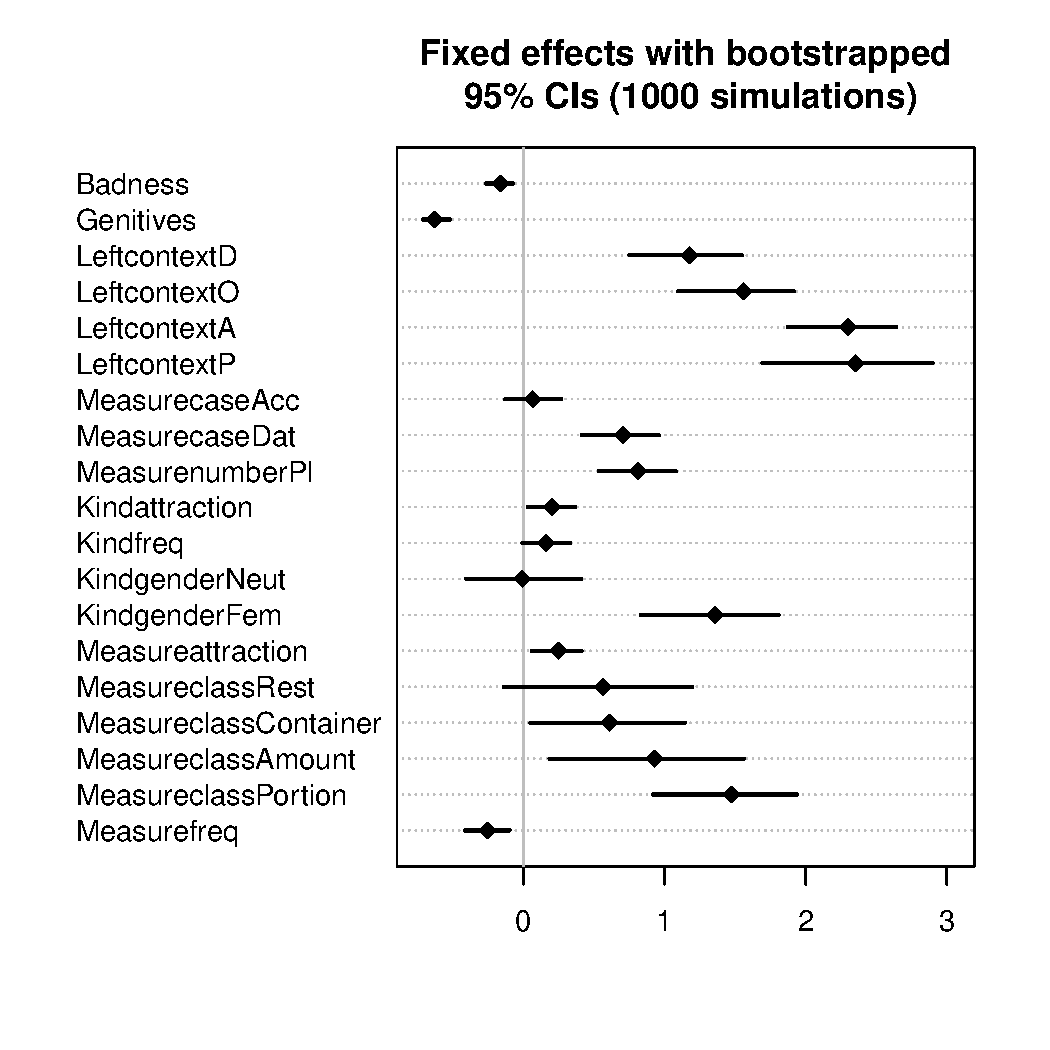
\includegraphics[width=0.85\textwidth]{../R/output/corpus_fixeffs}
  \caption{Coefficients with 95\% confidence intervals (for details see text); the intercept is -3.548}
  \label{fig:fixeffs}
\end{figure}

Then, a multilevel logistic regression model was fit which models the influence of the regressors specified in Table~\ref{tab:variables} on the probability that the \PGCa\ is chosen over the \NACa.
All regressors from Table~\ref{tab:variables} were included, and the measure lemma and the kind noun lemma were specified as varying-intercept random effects.
The sample size was \textit{n=}5,063 with 1,134 cases of \PGCa\ and 3,929 cases of \NACa.
The results of the estimation are shown in Table~\ref{tab:bigtable} and in Figure~\ref{fig:fixeffs}.
The intercept comprises \textit{Cardinal=Yes}, \textit{Measurecase=Nom}, \textit{Kindgender=Masc}, \textit{Measureclass=Physical}, and 0 for all numeric z-transformed regressors.
It was estimated at -3.548.

The regressors with the measure lemma as their unit of reference have no within-measure lemma variance, and the \textit{glmer} function automatically estimates them as group-level predictors (or second-level effects), cf.\ \citet[265--269,302--304]{GelmanHill2006} and Section~\ref{sec:itemandexemplareffects}.
The same goes for those listed with the kind lemma as their unit of reference.
Given the coding of the response variable, coefficients leaning to the positive side can be interpreted as favouring the \PGCa.

\begin{table}
  \centering
  \resizebox{\textwidth}{!}{
    \begin{tabular}{llrlrrrc}
    Model level  & Regressor         & $\text{p}_{\text{PB}}$ & Factor level & Coefficient & CI low & CI high & CI excludes 0 \\
    \midrule
    1               & Badness           &  0.002                 &              & -0.152      & -0.247 & -0.061  & *             \\
                    & Cardinal          &  0.001                 & No           &  1.189      &  0.862 &  1.466  & *             \\
                    & Genitives         &  0.001                 &              & -0.693      & -0.768 & -0.592  & *             \\
                    & Measurecase       &  0.001                 & Acc          &  0.030      & -0.150 &  0.212  &               \\
                    &                   &                        & Dat          &  0.705      &  0.455 &  0.944  & *             \\[0.5\baselineskip]
    
    2 (Kindlemma)   & Kindattraction    &  0.020                 &              &  0.225      &  0.049 &  0.393  & *             \\
                    & Kindfreq          &  0.095                 &              &  0.146      & -0.023 &  0.301  &               \\
                    & Kindgender        &  0.001                 & Neut         &  0.021      & -0.367 &  0.392  &               \\
                    &                   &                        & Fem          &  1.269      &  0.800 &  1.709  & *             \\[0.5\baselineskip]
    
    2 (Measurelemma & Measureattraction &  0.001                 &              &  0.282      &  0.106 &  0.447  & *             \\
                    & Measureclass      &  0.001                 & Container    &  0.252      & -0.265 &  0.788  &               \\
                    &                   &                        & Rest         &  0.421      & -0.209 &  1.063  &               \\
                    &                   &                        & Amount       &  0.831      &  0.215 &  1.432  & *             \\
                    &                   &                        & Portion      &  1.217      &  0.675 &  1.684  & *             \\
                    & Measurefreq       &  0.005                 &              & -0.231      & -0.363 & -0.079  & *             \\

  \end{tabular}
  }
  \caption{Coefficient table with 95\% bootstrap confidence intervals for the main study; the intercept is -3.548}
  \label{tab:bigtable}
\end{table}

Standard diagnostics show that the model quality is quite good.
Nakagawa \& Schielzeth's pseudo-coefficient of determination is $R_m^2=0.409$ and $R^2_c=0.495$.
The rate of correct predictions is 0.843, which means a proportional reduction of error of $\lambda=0.297$.
Generalised variance inflation factors for the regressors were calculated to check for multicollinearity \citep{FoxMonette1992,ZuurEa2010}, and the highest corrected $\text{GVIF}^{1/2\text{df}}$ was 1.520 for \textit{Cardinal}.
The lemma intercepts have standard deviations of $\sigma_{\text{Measurelemma}}=0.448$ and $\sigma_{\text{Kindlemma}}=0.604$.
Only \textit{Kindfreq} ($\mpPB=0.095$) could be seen as slightly too high to be convincing, failing at sig=0.05.

Using signed logarithmised collexeme strength (\textit{Measurecollo} and \textit{Kindcollo}) (with smoothing to avoid arithmetic problems) instead of the quotient for the attraction strength (\textit{Measureattraction} and \textit{Kindattraction}) (see Section~\ref{sec:variablesandannotation}) was not successful.
While the attraction measures reach satisfying sig levels in the PBmodcomp test (0.020 for \textit{Kindattraction} and 0.001 for \textit{Measureattraction}), the $p_{\text{PB}}$ value for \textit{Kindcollo} was 0.191 and the one for \textit{Measurecollo} was 0.443.
The coefficients of determination drop to $R_m^2=0.376$ and $R^2_c=0.480$.

\subsubsection{Interpretation}
\label{sec:mainstudyinterpretation}

\begin{figure}[h!]
  \centering
  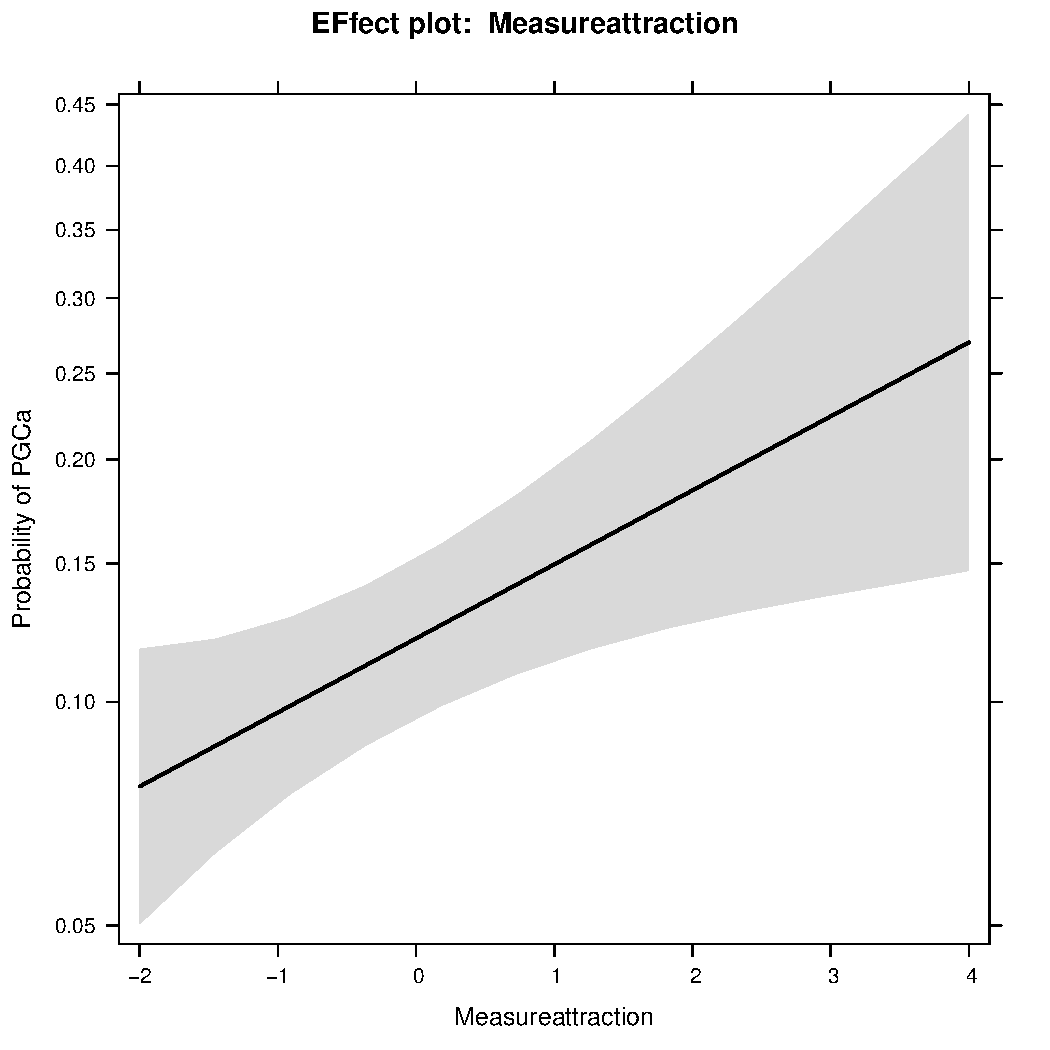
\includegraphics[width=0.5\textwidth]{../R/output/corpus_Measureattraction}~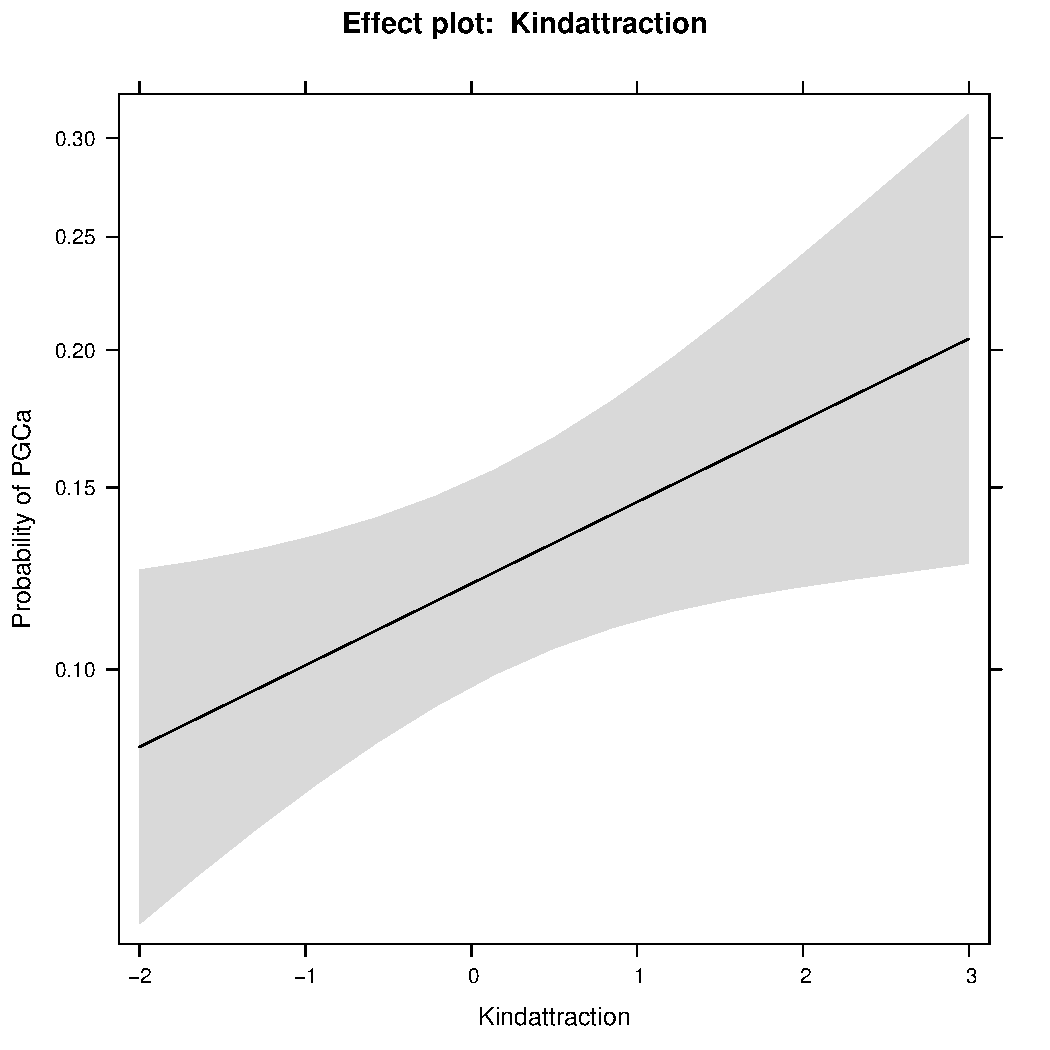
\includegraphics[width=0.5\textwidth]{../R/output/corpus_Kindattraction}
  \caption{Effect plots for the regressors \textit{Measureattraction} and \textit{Kindattraction}; y-axes are not aligned}
  \label{fig:eff:attraction}
\end{figure}

The results reported in Section~\ref{sec:corpushierarchicalmodel} generally confirm the hypotheses from Section~\ref{sec:analyses}.
First, the prototypicality effect related to the non-alternating \PGCd\ and \NACb\ can be shown (see the effect plots in Figure~\ref{fig:eff:attraction}).%
\footnote{Effect plots were created using the \textit{effects} package \citep{Fox2003}.}
The effect is as expected:
if a lemma appears relatively more often in the \PGCd\ (compared to its frequency in the \NACb), the \PGCa\ tends to be chosen over the \NACa\ with this specific lemma.
The effect for measure nouns is stronger, and it was estimated with higher precision.

An interesting picture emerges for the lemma frequencies.
A higher-than-average lemma frequency of measure nouns favours the \NACa, which is as expected if we assume at least a tendency for highly grammaticalised items to be more frequent.
With kind nouns, higher frequency seems to favour the \PGCa.
However, there is no clear theoretical interpretation (see Section~\ref{sec:analyses}), and the estimate is imprecise (not significant at sig=0.05).
The effect can therefore be ignored or treated as a nuisance variable.


\begin{figure}[h!]
  \centering
  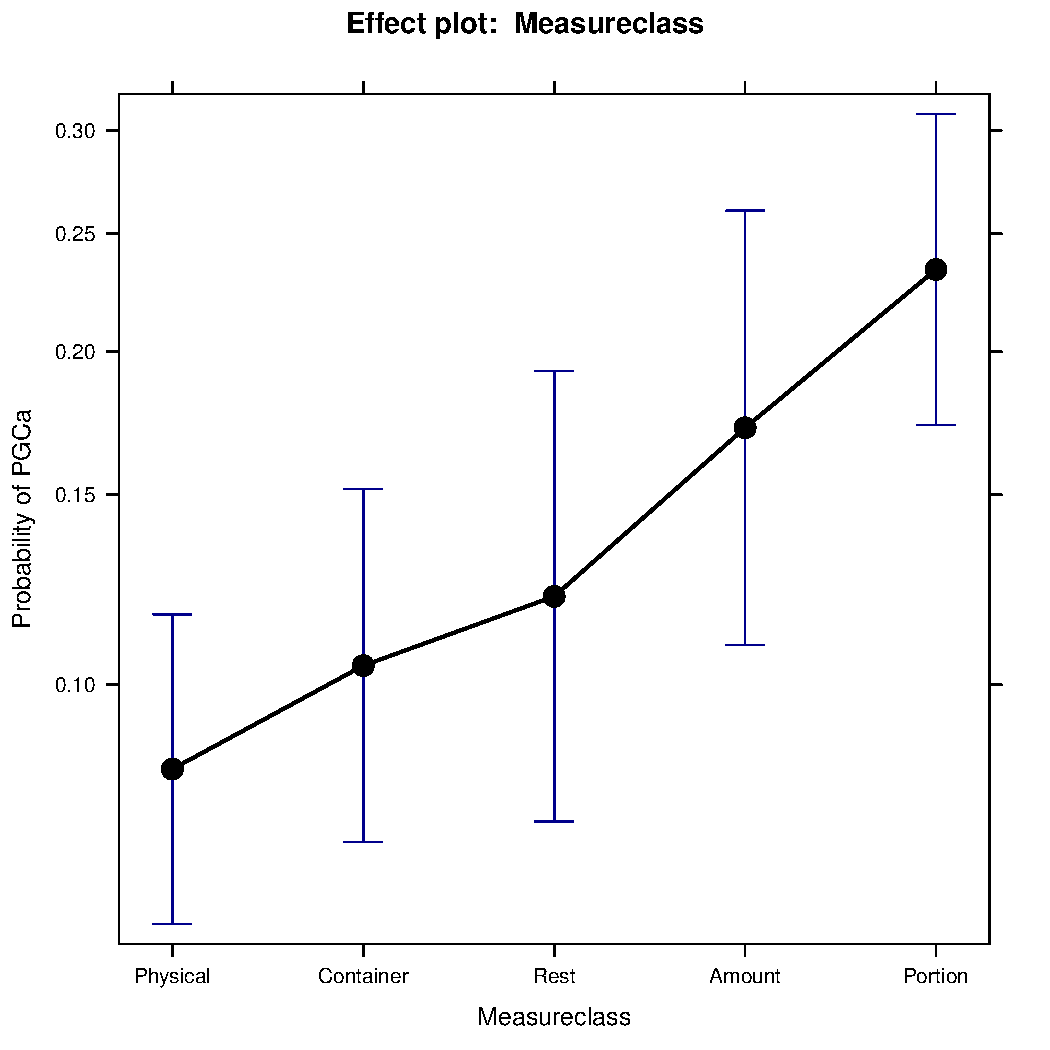
\includegraphics[width=0.5\textwidth]{../R/output/corpus_Measureclass}
  \caption{Effect plot for the regressor \textit{Measureclass}}
  \label{fig:eff:measureattraction}
\end{figure}

In Section~\ref{sec:analyses}, it was also hypothesised that classes of measure nouns with a higher degree of grammaticalisation should favour the \NACa.
The \textit{Measureclass} second-level predictor reaches sig=0.05 in the PBmodcomp test.
Looking at the effect plot in Figure~\ref{fig:eff:measureattraction}, it is evident that abstract non-referential physical measure nouns (such as \textit{Gramm} `gram' or \textit{Liter} `litre') with a high degree of grammaticalisation favour the \NACa.
At the other end of the scale, nouns denoting natural portions like \textit{Haufen} `heap', \textit{Bündel} `bundle', \textit{Schluck} `gulp' favour the \PGCa.
These are referential nouns, confirming the hypothesis that it is prototypical of the PGC to contain two referential nouns, while the NAC prototypically only contains one (the kind noun).

\begin{figure}[h!]
  \centering
  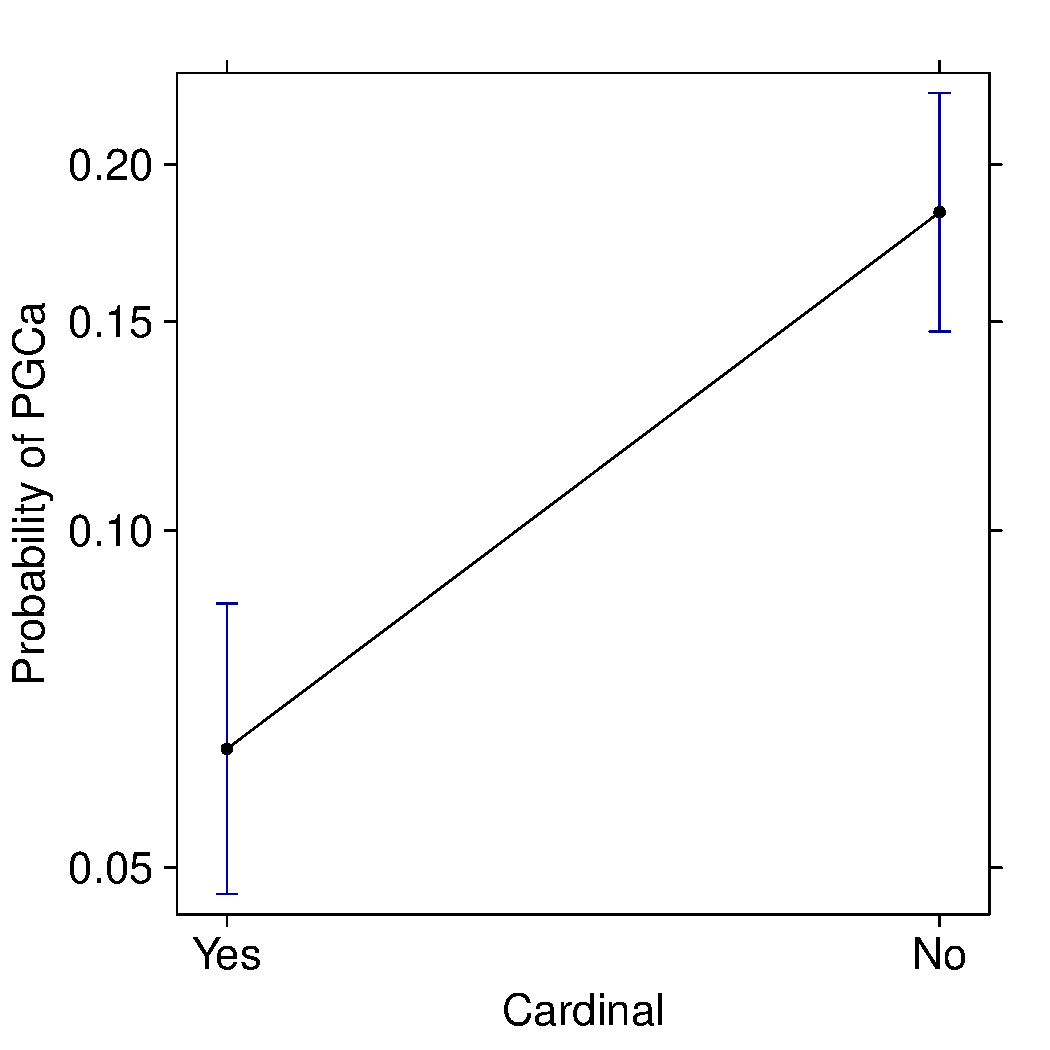
\includegraphics[width=0.5\textwidth]{../R/output/corpus_Cardinal}
  \caption{Effect plot for the regressor \textit{Cardinal}}
  \label{fig:eff:leftcontext}
\end{figure}

Figure~\ref{fig:eff:leftcontext} shows that cardinals indeed influence the choice of the alternant, and that cardinals have a strong tendency to co-occur with the \NACa.
This effect was predicted in Section~\ref{sec:analyses}.

The style-related proxy variables point in the expected direction.
Increased \textit{Badness} of the document favours the \NACa, and so does a lower density of genitives.
While these are merely proxies to style, this result can at least encourage future work into stylistic effects. 

The influence of \textit{Measurecase} is as predicted in previous analyses (see Section~\ref{sec:analyses}).
A measure noun in the dative favours the \PGCa\ (compared to the nominative, which is on the intercept).
Although \textit{Measurecase} is a nuisance variable in the context of this study, convergence with previous work strengthens its validity.

To close this section, I now compare the results of the pre-study and the main study.
Even though the non-alternating constructions are surely subject to additional constraints, the coefficients align neatly in many cases.
First of all, the intercepts encode a similar overall dominance of the NAC constructions (pre-study: -5.370; main study: -3.548).
For the \textit{Cardinal} effect, the coefficients 1.419 (pre-study) and 1.189 (main study) have the same sign and magnitude and mostly overlapping confidence intervals.
The levels of \textit{Measureclass} have comparable coefficients, although the divergence is larger.
In both studies, the non-referential measure nouns in the \textit{Physical} class (on the intercept) are most clearly associated with the NAC constructions.
Also, in both cases, the \textit{Container} class is closest to \textit{Physical} with the same sign and magnitude (pre-study: 0.445; main study: 0.252).
The main difference -- if we ignore the \textit{Rest} class which can be expected to show no clear tendency -- is that \textit{Amount} and \textit{Portion} are slightly closer together in their tendency to favour the PGC constructions in the pre-study (\textit{Amount} 1.597 and \textit{Portion} 1.782 in the pre-study vs.\ \textit{Amount} 0.831 and \textit{Portion} 1.217 in the main study).
The difference is not huge, and the overall order of the coefficients is the same.
The \textit{Genitives} effect also converges with -0.710 in the pre-study and -0.693 in the main study.
The two studies do not converge with respect to the \textit{Badness} variable, which is not significant in the pre-study.
It would, however, surprise to achieve perfectly converging results given that even real effects are missed at certain rates in empirical studies.
In the case of \textit{Badness}, we see that even in the main study, the effect size is small (-0.152), and thus even at the impressive sample size of roughly 5,000 in both studies, the effect might simply be too weak to be detected reliably.
Finally, the frequency effect \textit{Measurefreq} is detected in the main study but not in the pre-study, while the \textit{Kindfreq} effect is essentially absent in both studies.
In connection with this, it is revealing to look at the coefficients of determination.
In the pre-study, a much greater proportion of the variance is explained by taking the lemma random effects into account ($R^2_m=0.278$ and $R^2_c=0.566$) than it is in the main study ($R^2_m=0.376$ and $R^2_c=0.480$).
Thus, the frequency effect for measure lemmas might be swamped by the lemma random intercepts.
All things considered, the studies have shown that the predicted prototype effects are found in usage data for both the alternating and the non-alternating constructions.

\section{Experiments}
\label{sec:experimental}

\subsection{Experiment 1: forced-choice}
\label{sec:exp:fc}

\subsubsection{Setup, stimuli, and participants}

In the two experiments reported in this section, I use probabilities for the alternating constructions calculated for attested material, and I correlate these probabilities with the participants' reactions.
Thus, a direct link can be established between output material found in corpora and the behaviour of linguistic agents (see also Section~\ref{sec:cogocl}).
Both experiments use sentences containing attested MNPs from the corpus sample (embedded into simplified sentences) as stimuli.
Also, the probabilities that the corpus-based model assigns to the two alternants in these sentences are used as the main regressor in both studies.

The first experiment tests preferences for constructions explicitly.
\cite{FordBresnan2013} use the \textit{split-100} task in which participants have to distribute 100 points between the alternatives, assigning more points to more natural sounding alternative.
In essence, participants distribute a probability mass between two alternants, which is intended to produce more subtle results compared to a two-alternative forced-choice task such as in \cite{Rosenbach2013}, where participants have to choose one of two alternants.
The split-100 paradigm has been criticised in \cite{ArppeJaervikivi2007}.
The criticism was reiterated in \cite{DivjakEa2016}, where they use a forced-choice task.
In \cite{VerhoevenTemme2017}, it was shown that results from forced-choice and split-100 experiments mostly converge (with some numeric intricacies related to the non-linear distribution of preferences for alternants).
I present a forced-choice experiment in this Section instead of a split-100 experiment not only because of some researchers' critical attitude towards the split-100 task, but also because in a dry run of the experiment, participants complained about the unnaturalness of distributing a probability mass across two alternants and tended to produce ratings of 0 and 100 (and to a lesser degree 50).
Participants had to choose between two sentences that differed only in that one contained the \NACa\, and the other one contained the \PGCa.
The analysis compares the probabilities assigned to the stimuli by the corpus-derived model with the frequency with which participants chose the alternants for the same stimuli.

There were 24 participants (native speakers of German without reading or writing disabilities) aged 19 to 30 living permanently in Berlin, who were recruited from introductory linguistics courses at Freie Universität Berlin.
Although the experiment was conducted in the last four weeks of their first semester, participants had no deeper explicit knowledge of linguistics, grammar, or experimental methods.
None of them had ever participated in a forced-choice experiment before.
Participation was voluntary but participants received credit in partial fulfillment of course requirements.

As stimuli, attested MNPs from the corpus study were used, but the sentences were radically simplified to avoid influences from contextual nuisance factors as much as possible.
The approach is also justified because according to the theoretical assessment in Section~\ref{sec:analyses}, the choice of alternants depends mostly on a very local constructional context.
I sampled 16 MNPs from the concordance and made sure that the simplifications and normalisations did not affect any of the regressors used in the corpus study.
In the simplified sentences, the case, number, etc. of the MNP remained the same as in the attested sentence, as did the choice of lexical material within the MNP.
Eight sentences contained masculine or neuter kind nouns, and the other eight contained feminine kind nouns.
Furthermore, in each of the masculine\slash neuter and feminine groups, four sentences originally containing the \NACa\ and four sentences originally containing the \PGCa\ were chosen.
More precisely, the sentences were sampled as \textit{highly typical examples} of \PGCa\ (high probability assigned by GLMM) and \NACa\ (low probability assigned by GLMM), respectively.%
\footnote{Remember from Section~\ref{sec:corpusstudies} that the model predicts the probability that the \PGCa\ is chosen over the \NACa.}
High and low probabilities were defined as the top and bottom 20\% of all probabilities assigned by the GLMM.
Lemmas and feature combinations were made unique within each group whenever possible.
The design is summarised in Table \ref{tab:experiment1:design}.

\begin{table}
  \centering
  \begin{tabular}[h]{lll}
     & Masculine\slash Neuter & Feminine \\
     \midrule
     \textbf{high prob.\ for PGC\Subsf{adj}} & 4 sentences & 4 sentences \\
     \textbf{low prob.\ for PGC\Subsf{adj}} & 4 sentences & 4 sentences \\
  \end{tabular}
  \caption{The four groups of sentences chosen as stimuli; in each group of four sentences, combinations of important factor values were made unique whenever possible}
  \label{tab:experiment1:design}
\end{table}

The final pairs of stimuli were the sentence containing the attested and preferred alternant (according to the corpus GLMM) on the one hand and a modified version containing the dispreferred alternant on the other hand.
They were presented next to each other, and a 20 second time limit for each choice was set.%
\footnote{No participant ever exceeded the time limit.}
The position on the screen (left\slash right) and the order of sentences were randomised for each participant.
As fillers, 23 pairs of sentences exemplifying similar but unrelated alternation phenomena from German morpho-syntax were used.
Thus, participants saw 39 pairs of sentences and 78 sentences in total.
They were instructed to select from each pair of sentences the one that seemed more natural to them in the sense that they would use it rather than the other one.
The experiment was conducted using \textit{PsychoPy} \citep{Peirce2007}.

\subsubsection{Model}

\begin{figure}[htbp!]
\centering
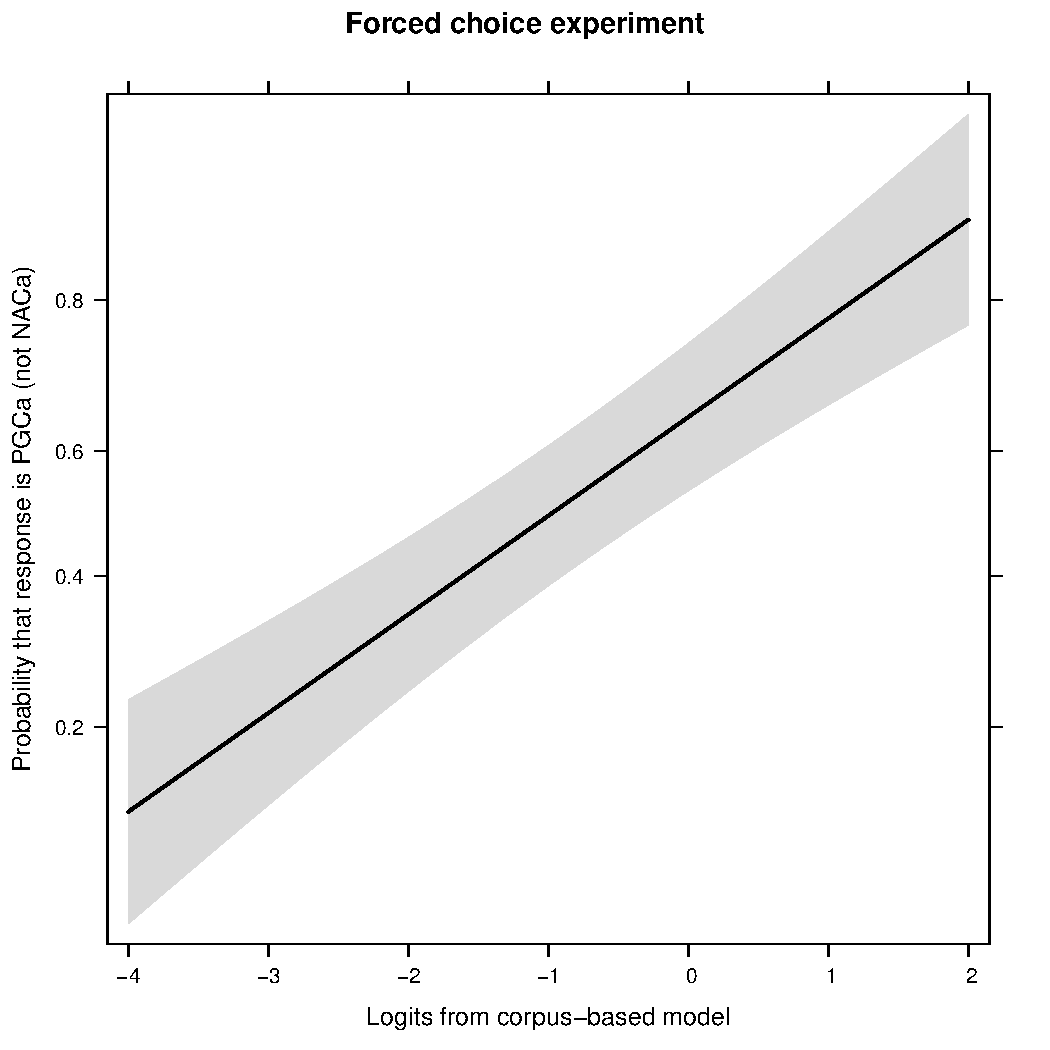
\includegraphics[width=0.5\textwidth]{../R/output/fc_effects}
\caption{Effect plot for the multilevel logistic regression in the forced-choice experiment: predictability of participants' choices using the probabilities derived from the corpus-based GLMM}
\label{fig:afc:effects}
\end{figure}

A multilevel logistic regression was specified with the probability of the \PGCa\ predicted for each sentence by the corpus-based GLMM as the only fixed effect \textit{Modelprediction}.%
\footnote{The document-level variables \textit{Badness} and \textit{Genitives} were set to 0, which is the mean for z-transformed variables.}
A random intercept and slope were added for the individual sentence (item) in order to catch idiosyncrasies of single sentences.
Coefficients were estimated with Maximum Likelihood Estimation (\textit{lmer} function from \textit{lme4}).
The number of observations was \textit{n=}384.

\begin{figure}[htbp!]
  \centering
  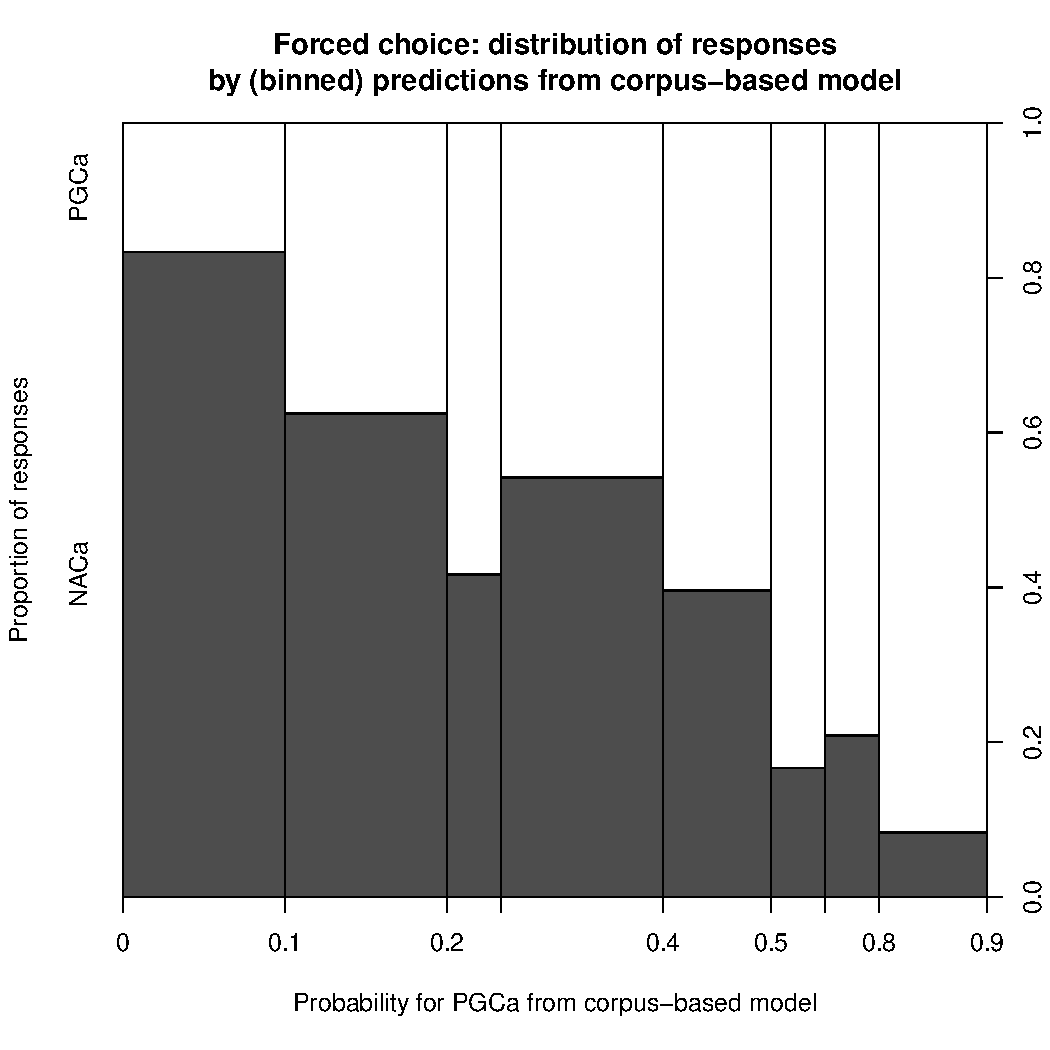
\includegraphics[width=0.5\textwidth]{../R/output/fc_proportions}
  \caption{Spineplot of the proportion of responses plotted against the predictions from the corpus-based model in the forced-choice experiment}
  \label{fig:spines}
\end{figure}

A good amount of the variance can be accounted for by idiosyncrasies of single sentences ($\sigma_{\text{Item}}=1.217$).%
Also, among participants, there are clearly different preferences ($\sigma_{\text{Participant}}=0.412$).
On the extreme ends, one participant chose the \PGCa\ in 13 of 16 cases, and two participants only chose it in 5 of 16 cases.
The regressor \textit{Modelprediction} achieves $\mpPB=0.003$ (1,000 replications) and is estimated at 4.389 relative to an intercept of -1.270.
The confidence interval from a parametric bootstrap (1,000 replications, percentile method) for the regressor is acceptable but slightly large with a lower bound of 1.788 and an upper bound of 6.599.
The pseudo-coefficients of determination are $R^2_{m}=0.185$ and $R^2_{c}=0.455$, which means that roughly 19\% of the variance in the data can be explained by considering only the predictions from the corpus-based GLMM.

\subsubsection{Interpretation}

The coefficients of determination indicate a weak result for the fixed effects part, which is nonetheless worthy of mention (very close to 0.2).
The effect display for the single fixed regressor \textit{Modelprediction} is given in Figure \ref{fig:afc:effects}.
The higher the probability of the \PGCa\ predicted from usage data, the more often participants chose the \PGCa\ alternant in the forced-choice task.
A closer look at the results in the form of the spineplot in Figure~\ref{fig:spines} shows, however, that it was likely idiosyncracies in the sentences with a model prediction between 0.5 and 0.6 which spoiled an otherwise much better correlation.
Clearly, a revised and improved experiment might lead to a much better fit in future research.

In principle, a per-stimulus random effect for \textit{Modelprediction} could also remedy the problem with individual stimuli at least partially.
Therefore, a model with random slopes for \textit{Modelprediction} and both random effects (\textit{Participant} and \textit{Item}) was specified and estimated.
The random slope for participants was added to comply with \citet[257]{BarrEa2013} who predict \textit{catastrophically high Type I error rates} for experimental designs with within-subject manipulations if random effects structures are not kept maximal.
The coefficient of the fixed effect changed noticeably but not enough to change the interpretation (5.408 relative to an intercept of -1.304), and the marginal $R^2_m$ rises to 0.213 ($R^2_c=0.488$).
In line with expectations, the standard deviation in the random slopes for \textit{Item} is high at 5.996.
However, the covariance parameters were estimated at -1.0, which is a clear sign that the variance-covariance matrix could not be estimated successfully.
The same was true for models with only \textit{Item} and \textit{Participant} random slopes.
This is exactly the kind of model overparametrisation criticised in \citet{BatesEa2015a} and \citet{MatuschekEa2017}.
The available data is simply insufficient to estimate the parameters of the more complex model with varying slopes.%
\footnote{\citet[1]{BatesEa2015a} state: ``We show that failure to converge typically is not due to a suboptimal estimation algorithm, but is a consequence of attempting to fit a model that is too complex to be properly supported by the data, irrespective of whether estimation is based on maximum likelihood or on Bayesian hierarchical modeling with uninformative or weakly informative priors.
Importantly, even under convergence, overparameterization may lead to uninterpretable models.''
}

In summary, the forced-choice experiment succeeded in corroborating the results from the corpus study in as much as the preferences extracted from usage data correspond to native speakers' choices, but the correlation is weak, likely due to problems with individual test items and\slash or too few data.


\subsection{Experiment 2: self-paced reading}
\label{sec:exp:spr}

\subsubsection{Setup, stimuli, and participants}

The second experiment tests preferences more implicitly.
It is expected that reading less typical alternants (the one assigned a low probability by the corpus-derived model) in a given context and with given lexical material incurs a processing overhead for the reader (\citealp{Kaiser2013}).
In this section, a self-paced reading experiment is therefore presented.
In a very similar fashion, \cite{DivjakEa2016} apply the self-paced reading paradigm in the validation of corpus-based models.
The analysis compares the corpus-derived probabilities with potential lags in reading time for sentences with the preferred and the non-preferred constructions.

Concretely, the exact same stimuli as in the forced-choice experiments were used.
Each participant read both the 16 sentences with the alternant predicted by the corpus model and the 16 modified sentences with the alternant that the corpus model did not predict.%
\footnote{Notice that lemmas and their frequencies as well as lemma classes are included as regressors in the corpus-based GLMM, and there was consequently no additional controlling of lemma frequencies, etc.}
To minimise repetition effects, the stimuli for each participant were separated into two blocks of 16 targets and 33 fillers per block.
In the experiment, participants first read all sentences from the first block, then all sentences from the second block.
From each target sentence pair, one sentence was assigned to the first block and the other sentence to the other block.
The assignment of members of the individual sentence pairs to the blocks was randomised for each participant individually, as was the order within each block.
The sentences from each pair of alternants were kept as far apart as possible.
The fillers also came in pairs such that the second block exclusively contained sentences to which participants had been exposed in the first block in slightly modified form.
In total, each participant read 98 sentences.
After each sentence, participants had to answer simple (non-metalinguistic) yes-no questions about the previous sentence as distractors.
The distractor questions were different between the first and the second blocks.
There were 38 participants recruited in exactly the same manner as for the experiment reported in Section~\ref{sec:exp:fc}.
None of them had ever participated in any kind of reading experiment, and none of them took part in the first experiment.
The experiment was conducted using \textit{PsychoPy}.

The reading times were residualised per speaker based on the reading times of all words (not just the targets) by that speaker.
The adjective and the kind noun (\ie\ the constituents bearing the critical case markers) were used as the target region, for instance the bracketed words in the example \textit{zwei Gläser} [\textit{spru\-deln\-des Wasser}] `two glasses of sparkling water'.
Outliers farther than 2 inter-quartile ranges from the mean logarithmised residualised reading time were removed (64 data points), resulting in a total number of \textit{n=}1,152 observations.

\subsubsection{Model}

An LMM was specified with the logarithmised residual reading times as the response variable.
The probabilities derived from the corpus GLMM (\textit{Modelprediction}) were added as the main regressor of interest.
It should be remembered that the corpus GLMM predicts the probability of the \PGCa.
As a consequence, the higher the GLMM prediction is, the more typical the sentence is for containing the \PGCa.
It is therefore expected that reading times are higher when the value of \textit{Modelprediction} is higher but the sentence contains the \NACa.
However, when the sentence contains the \PGCa, reading times should be lower when \textit{Modelprediction} is higher.
To account for this, an interaction between \textit{Modelprediction} and \textit{Construction} (levels \textit{PGCadj} and \textit{NACadj}) was added to the model.

Furthermore, the position (1--98) of the sentence in the individual experiment (\textit{Position}) was included as a fixed effect to control for the usual increase in reading speed during an experiment run.
Random intercepts were specified for \textit{Participant} and \textit{Item} (the 16 sentence pairs are one \textit{Item} each).%
\footnote{Again, all attempts to include random slopes resulted in the variance-covariance matrix not being properly estimated (1 or -1 covariance parameters).}

\begin{table}
  \centering
  \begin{tabular}{lrrrc}
    Regressor & \multicolumn{1}{r}{Coefficient} & \multicolumn{1}{r}{CI low} & \multicolumn{1}{r}{CI high} & \multicolumn{1}{r}{CI excludes 0} \\ \midrule
    Construction=PGCadj                 &  0.054 &  0.012 &  0.095 &  *  \\ 
    Modelprediction                     & -0.003 & -0.113 &  0.110 &     \\ 
    Position                            & -0.005 & -0.005 &  0.004 &     \\ 
    Construction=PGCadj:Modelprediction & -0.125 & -0.234 & -0.023 &  *  \\ 
  \end{tabular}
  \caption{Fixed effect coefficient table for the LMM used to analyse the self-paced reading experiment; the intercept is 0.829}
  \label{tab:exp:spr}
\end{table}

Table~\ref{tab:exp:spr} shows the coefficient estimates with a 95\% parametric bootstrap confidence interval (1,000 replications, percentile method).
The standard deviation of the participant intercepts is $\sigma_{\text{Participant}}=0.079$ and of the item intercepts $\sigma_{\text{Item}}=0.037$.
Comparing the full model to a model without the main regressor \textit{Modelprediction} (and consequently also without the interaction with \textit{Construction}) in a PB test gives $\mpPB=0.036$.
The pseudo-coefficients of determination are $R^2_m=0.239$ and $R^2_c=0.346$.

An alternative Gaussian generalised additive model with an identity link was also fit (see \citealp{DivjakEa2016}) using the \textit{mgcv} package \citep{Wood2011}.
The full results are included in the data package for this paper, but the fit was not better than with the LMM reported above.
The estimated smoother for the \textit{Modelprediction} variable is essentially linear, and the $R^2$ (corresponding to the marginal $R^2$ of the LMM) was 0.237.

\subsubsection{Interpretation}

The coefficients of determination indicate that there is a noteworthy correlation between the reactions of the subjects and the corpus-derived probabilities (marginal $R^2$ and that there some inter-subject variation (conditional minus marginal $R^2$).

\begin{figure}[htbp!]
\centering
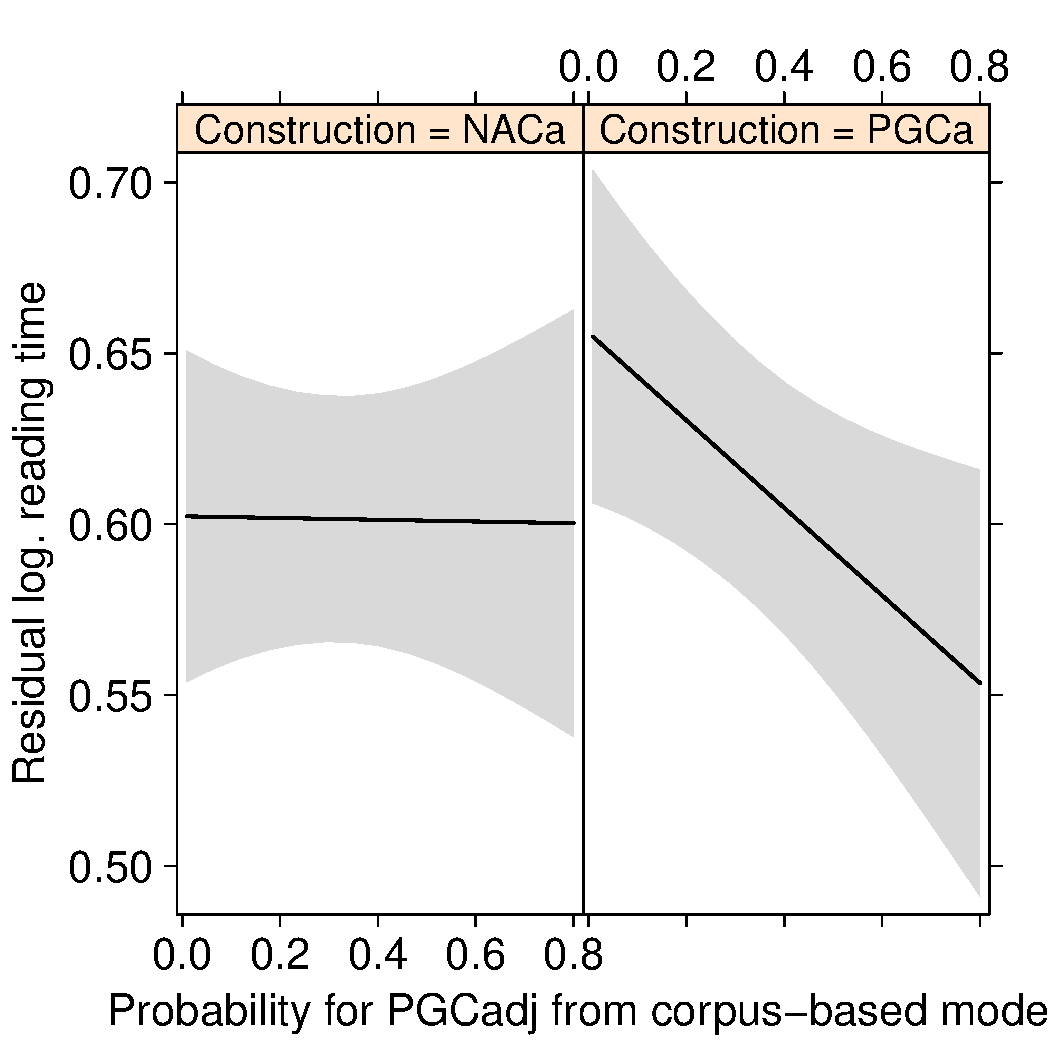
\includegraphics[width=0.5\textwidth]{../R/output/spr_effects}
\caption{Effect plot for the LMM in the self-paced reading experiment: modeling participants' residualised log reading times on the probabilities given by the corpus-based GLMM}
\label{fig:spr:effects}
\end{figure}

The effect plot for the interaction of interest is shown in Figure~\ref{fig:spr:effects}.
The estimate for the sentences with \NACa\ is obviously imprecise and no significant differences in reading times are observed.
There is a clearer effect in the sentences with \PGCa, which is also confirmed by the significant results from the bootstrapped confidence intervals (see Table~\ref{tab:exp:spr}) and from the PB test reported above.
The \PGCa\ brings about an increased reading time, which is plausible because it is the much rarer construction (see Section~\ref{sec:corpusstudies}).
However, if it occurs in a prototypical context and with prototypical lexical material, reading times drop.
This can be seen in the downward slope in the right panel of Figure~\ref{fig:spr:effects}.
This fits into the general picture inasmuch as the construction with the lower frequency might be developing towards a more sharply defined prototype.%
\footnote{In this context, it should be remembered from Section~\ref{sec:corpusstudies} that even the \PGCd\ is much rarer that the \NACb\ (17,252 vs.\ 315,635 occurrences in the auxiliary corpus samples).}
Conversely, the \NACa\ (like the NAC in general) might be the highly frequent default which does not incur a reading time penalty, even if it is not the optimal choice in the given context and with the given lexical material.

In Section~\ref{sec:conclusion}, I take stock and summarise the contribution of the present study to the research on alternations in cognitive linguistics.

\section{Conclusions}
\label{sec:conclusion}

\hl{Mention pre-registration.}

This paper stands in a now ten year-old tradition of research on grammatical alternations using corpus and experimental data.
In my view, the main tenets of this line of research are:
(i)~Language, viewed from a cognitively realistic angle, is a probabilistic phenomenon and cannot be modelled appropriately within Aristotelian frameworks that assume discrete categories.
(ii)~Corpora are collections of usage events (language production) and can therefore be used to evaluate both the claim made in (i) and specific theoretical claims (in case studies) about factors influencing speakers' decisions to use specific forms or constructions.
(iii)~Given (ii), we expect results from corpus analyses and from appropriate experiments to yield similar results, not necessarily as a form of validation of the corpus-based findings, but as converging evidence.
I consider these three points to be of utmost importance because they clearly set this approach to linguistic research apart from \textit{both} Aristotelian frameworks \textit{and} introspective, non-empirical, and anti-quantitative versions of cognitive linguistics (see \citealp{Dabrowska2016} for a pithy philippic against such approaches).

The present paper adds to the evidence that all of the aforementioned three points are correct.
A grammatical alternation in German measure NPs was examined using corpus data based on factors partly derived from existing accounts, formulated in terms of construction prototypes.
The preferences extracted from the DECOW web corpus were confirmed in a forced-choice experiment, in which participants explicitly chose alternants in line with the probabilities derived from the corpus-based model.
In a more implicit self-paced reading experiment, it was shown that the much rarer alternant brings about a reading time penalty except in cases for which the corpus model predicts very high probability for this alternant.

Future work could extend these results and provide a general picture of the constructions expressing measurements (see Section~\ref{sec:descriptive}).
This would be a much more complicated task given that the choices then would no longer be binary and that the meaning of the alternative ways of expressing measurements are semantically more varied.
Finally, I want to point out that German is mildly under-researched in the specific framework used here.
This is quite surprising given the fact that German morpho-syntax is famous for its alternations, which are usually called \textit{Zweifelsfälle} (`cases of doubt') in the traditional literature \citep{Duden09,Klein2009}.
Instead of being drowned in normative, descriptive, or didactic discussions, they could serve as ideal test cases in cognitive linguistics.






\begin{acknowledgement}
  I thank (in alphabetical order) Felix Bildhauer, Susanne Flach, Elizabeth Pankratz, Samuel Reichert, Ulrike Sayatz, and Christian Zimmer for valuable discussions and comments.
  Also, I would like to thank the three reviewers for Cognitive Linguistics as well as associate editor Dagmar \mbox{Divjak} for insightful comments which helped to improve the quality of this paper significantly.
  Furthermore, I thank Ulrike Sayatz for helping me to recruit the participants for the experiments.
  I am grateful to Sonya Faber and Elizabeth Pankratz (in alphabetical order) for fixing my English.
  Finally, I am grateful to my student assistants Kim Maser for her work on the annotation of the concordances and Luise Rißmann for supervising most of the experiments.
  The research presented here was made possible in part through funding from the \textit{Deutsche Forschungsgemeinschaft} (DFG, personal grant SCHA1916/1-1).
\end{acknowledgement}


\bibliography{rs}

\end{document}

